\documentclass[12pt,titlepage,headings,oneside,openany]{book}
\usepackage{kotex}
\usepackage{graphicx}
\usepackage{epsfig}
\usepackage{epstopdf}
\usepackage{subfigure}
\usepackage{rotating}
\usepackage{enumitem}
\usepackage{amsfonts,amssymb}
\usepackage{pifont}
\usepackage{indentfirst}
\usepackage{lscape}
\usepackage{booktabs,longtable,adjustbox,caption,array}
\usepackage{soul}
\soulregister{\ref}{1}
\soulregister{\cite}{1}
\usepackage{xcolor}
\usepackage{fvextra}
\usepackage{algorithmic}
\usepackage{stfloats}
\usepackage{verbatim}
\usepackage[cmex10]{amsmath}
\usepackage{newlfont}
\usepackage{XThesis_skku_eng}
\usepackage[active]{srcltx}
\usepackage{notebook}
\usepackage{fancyhdr}
\usepackage{cite}
\usepackage[hyphens]{url}
\usepackage{array,tabularx}
\usepackage{bm,upgreek}
\usepackage{textcomp}
\usepackage{makecell,multirow}
\usepackage{ifpdf}
\usepackage{float}
\usepackage{placeins}
\usepackage{mathtools}
\usepackage{microtype}
\ifpdf
  \usepackage[CJKbookmarks]{hyperref}
  \hypersetup{hidelinks}
\else
  \usepackage[dvipdfm,CJKbookmarks]{hyperref}
  \hypersetup{hidelinks}
  \AtBeginDvi{\special{pdf: tounicode KSCms-UHC-UCS2}}
\fi
% Symmetric vertical margins for the thesis body.
% The previous template used a large positive \voffset and the default book-class
% chapter spacing, which pushed chapter titles far below the top of the page.
\usepackage[
  a4paper,
  top=25mm,
  bottom=25mm,
  left=36mm,
  right=36mm,
  includefoot,
  footskip=10mm
]{geometry}

% Place chapter headings at the top of the text area instead of adding the
% default 50 pt blank space used by the book class.
\makeatletter
\def\@makechapterhead#1{%
  \vspace*{0pt}%
  {\parindent \z@ \raggedright \normalfont
    \ifnum \c@secnumdepth >\m@ne
      \if@mainmatter
        \huge\bfseries \@chapapp\space \thechapter
        \par\nobreak
        \vskip 14\p@
      \fi
    \fi
    \interlinepenalty\@M
    \Huge \bfseries #1\par\nobreak
    \vskip 28\p@
  }}
\def\@makeschapterhead#1{%
  \vspace*{0pt}%
  {\parindent \z@ \raggedright \normalfont
    \interlinepenalty\@M
    \Huge \bfseries #1\par\nobreak
    \vskip 28\p@
  }}
\makeatother
\hfuzz2pt
\newlength{\defbaselineskip}
\setlength{\defbaselineskip}{\baselineskip}
\newcommand{\setlinespacing}[1]{\setlength{\baselineskip}{#1 \defbaselineskip}}
\newcommand{\doublespacing}{\setlength{\baselineskip}{2.0 \defbaselineskip}}
\newcommand{\singlespacing}{\setlength{\baselineskip}{\defbaselineskip}}

\usepackage{tikz}
\usetikzlibrary{arrows.meta,positioning,fit,calc,shapes.geometric}
\tikzset{block/.style={draw=black!65,rounded corners=2pt,align=center,fill=blue!4,inner sep=6pt,font=\small},
 link/.style={-{Latex[length=2mm]},thick},note/.style={align=center,font=\footnotesize}}
\newcommand{\thesistitle}{Human-Guided Local Robotic Polishing via Joint Motion--Force Representation and Force-Conditioned Imitation Learning}
\newcommand{\thesistitlekr}{인간의 영역 지정과 동작--힘 결합 표현 및 힘 조건부 모방학습을 활용한 국소 로봇 폴리싱}
\newcommand{\vect}[1]{\bm{#1}}
\newcommand{\R}{\mathbb{R}}
\newcommand{\NA}{\textemdash}
\expandafter\def\csname short@fig:mark_example\endcsname{Marked local region and registration}
\expandafter\def\csname short@fig:faire_architecture\endcsname{System overview and module interfaces}
\expandafter\def\csname short@fig:apparatus\endcsname{Archived robot apparatus photograph}
\expandafter\def\csname short@fig:teaching_frames\endcsname{Actual teaching-camera frames}
\expandafter\def\csname short@fig:demo_transfer\endcsname{Coordinate-processing chain}
\expandafter\def\csname short@fig:force_processing\endcsname{Recorded force-processing stages}
\expandafter\def\csname short@fig:dataset_split\endcsname{Episode lengths and dataset partition}
\expandafter\def\csname short@fig:teaching_motion_force\endcsname{Representative motion--force teaching}
\expandafter\def\csname short@fig:force_history_policy\endcsname{Implemented policy architecture}
\expandafter\def\csname short@fig:execution_architecture\endcsname{Command processing and contact execution}
\expandafter\def\csname short@fig:e1_primary_metrics\endcsname{E1 completion and excess-force results}
\expandafter\def\csname short@fig:e1_force_all\endcsname{All E1 measured force traces}
\expandafter\def\csname short@fig:e1_xy_all\endcsname{All E1 measured XY trajectories}
\expandafter\def\csname short@fig:e1_height_reference\endcsname{E1 exit-height reference sensitivity}
\expandafter\def\csname short@fig:e2_primary_metrics\endcsname{E2 timing, force peaks, and travel}
\expandafter\def\csname short@fig:e2_force_all\endcsname{All E2 measured force traces}
\expandafter\def\csname short@fig:e2_transition_cases\endcsname{E2 A4 and B4 transition cases}
\expandafter\def\csname short@fig:e1_photos\endcsname{First-run E1 initial and final snapshots}
\expandafter\def\csname short@fig:e2_sequence\endcsname{Frames from the first E2 C video}
\expandafter\def\csname short@fig:diagnostic_heatmap\endcsname{Uncalibrated execution heatmap}
\newcommand{\figfull}[3]{\begin{figure}[tbp]\centering\includegraphics[width=\linewidth]{figures/#1}\caption[\csname short@#3\endcsname]{#2}\label{#3}\end{figure}}
\captionsetup{font=small,labelfont=bf}
\newcolumntype{P}[1]{>{\raggedright\arraybackslash}p{#1}}
\renewcommand{\tabularxcolumn}[1]{P{#1}}
\renewcommand{\arraystretch}{1.15}
\setcounter{tocdepth}{1}
\setcounter{secnumdepth}{2}
\hypersetup{pdftitle={Human-Guided Local Robotic Polishing},pdfsubject={Revised master's thesis draft}}

\begin{document}
\setlinespacing{1.7}
\def\baselinestretch{1}
\pagestyle{fancy}\fancyhf{}\fancyfoot[C]{\thepage}
\renewcommand{\headrulewidth}{0pt}\renewcommand{\footrulewidth}{0pt}

\begin{titlepage}
\centering
{\large Master's Thesis\par}
\vspace{1.2cm}
{\fontsize{17.28}{23}\selectfont\bfseries\thesistitle\par}
\vspace{0.9cm}
{\large\thesistitlekr\par}
\vspace{1.3cm}
{\large Revised Draft\par}
\vfill
{\large The Graduate School\par}
\vspace{0.2cm}
{\Large Sungkyunkwan University\par}
\vspace{0.2cm}
{\large Department of Intelligent Robotics\par}
\vspace{1cm}
{\small Author and submission information: TBD\par}
\end{titlepage}

\pagenumbering{roman}
\tableofcontents\clearpage
\phantomsection\addcontentsline{toc}{chapter}{List of Tables}\listoftables\clearpage
\phantomsection\addcontentsline{toc}{chapter}{List of Figures}\listoffigures\clearpage
\chapter*{Abstract}
\addcontentsline{toc}{chapter}{Abstract}
\begin{center}\large\bfseries\thesistitle\end{center}

Surface finishing often requires local rework around a selected region rather than uniform treatment of an entire component. A local polishing operation must coordinate tool movement, contact force, and processing time within that region. In the setting considered here, a person specifies the region to be treated, avoiding dependence on autonomous recognition of fine scratches with the available equipment. This spatial instruction identifies where processing should occur but leaves the motion--force sequence to be constructed. Rules and demonstration replay provide legitimate solutions; the research question is when observation-conditioned skill generation provides additional execution value.

This thesis develops a human-guided local polishing framework that connects region specification with temporally paired motion--force demonstrations. A tracked teaching system records tool pose, three-axis interaction force, and RGB observations. Task-centered position learning is paired with an implemented direction-alignment adapter that maps observations into the teaching frame and restores generated XY paths. A conditional Flow Matching policy generates sequences of position, orientation, and target force from images, robot state, and measured-force history. A shared execution layer restores task coordinates, connects plans, and conditions commands before an existing lower-level force controller regulates contact. Skill generation, contact regulation, and procedural completion evaluation have distinct responsibilities.

Two robot evaluations examine this division, with direction alignment disabled. E1 compares rule-based planning, force-inclusive demonstration replay, and the force-conditioned policy under a nominal local task. All retained executions show the required loaded traversal. The original completion-rate differences are sensitive to the height reference used to recognize exit, while the learned policy exhibits greater excess-force exposure than the other providers. A separate replay analysis clarifies this sensitivity; physical height-variation trials remain planned. E2 separates learned target-force output from measured-force observation. The force-observing policy has shorter operator-terminated intervals in the recorded cohort, while one motion-only attempt remains in contact and is interrupted. These observations demonstrate an executable motion--force skill representation and reveal differences in phase progression, without establishing universal policy superiority or measured surface-quality improvement. The resulting framework supports a task-centered assessment of learning alongside rules and replay.

\vspace{0.4cm}
\noindent\textbf{Keywords:} Local Robotic Polishing, Human Task Specification, Motion--Force Skill, Imitation Learning, Flow Matching, Contact-Task Evaluation

\chapter*{Notation and Terminology}
\addcontentsline{toc}{chapter}{Notation and Terminology}
\begin{longtable}{P{0.23\textwidth}p{0.69\textwidth}}
\toprule Symbol & Meaning \\ \midrule
\endhead
\(B,V,T,E\) & Robot-base, VR tracking, tracker, and calibrated tool/TCP frames. \\
\({}^{B}T_E\) & Homogeneous pose of frame \(E\) in frame \(B\). \\
\(p,\rho,R\) & Position (mm), rotation vector (rad), and its rotation matrix. \\
\(c\in\R^2\) & Fixed task-origin XY coordinates in the robot base (mm). \\
\(\theta_{\mathrm{live}},\theta_{\mathrm{ref}},\alpha\) & Live stain-axis angle, teaching reference angle, and their wrapped alignment angle (rad). \\
\(R_2(\alpha),u\) & Planar rotation matrix and center-relative XY position aligned with the teaching direction (mm). \\
\(q=[p^\mathsf{T},\rho^\mathsf{T}]^\mathsf{T}\) & Six-dimensional Cartesian pose; the code name \texttt{qpos} does not denote joint angles here. \\
\(f^{\mathrm{demo}},f^{\mathrm{meas}}\) & Recorded teaching force and measured robot force (N). Superscripts identify their roles; frames are stated separately. \\
\(f^{\pi},f^{\mathrm{sent}},f^{\mathrm{applied}}\) & Policy-predicted, executor-transmitted, and controller-applied target forces (N). The last is not available as a synchronized recorded time series. \\
\(I_k,o_k\) & RGB observation and complete policy observation at physical sample \(k\). \\
\(a_k,A_k\) & One action and a future action sequence. \\
\(H,L\) & Action horizon (128 samples) and force-history length (30 samples) for the evaluated checkpoints. \\
\(t,k,\Delta t\) & Physical elapsed time (s), sample index, and physical sample interval. \\
\(s,z_s,v_\theta\) & Dimensionless flow time, noisy normalized action sequence, and learned vector field. \\
\(g(t)\) & Operational contact gate from measured robot-base \(F_z\). \\
\(Q_{95},J_{\mathrm{excess}}\) & Common teaching base-force reference (N) and excess-force integral (N\,s). \\
\(R,T,C\) & E1 rule, teaching replay, and force-conditioned learned providers. \\
\(A,B,C\) & E2 motion-only, learned motion--force without force observation, and learned motion--force with force observation. \\
\bottomrule
\end{longtable}

\emph{Task specification} identifies the local region and task setting. A \emph{motion--force skill} is a temporally organized sequence of pose and target-force references. \emph{Contact regulation} is the lower-level response to force feedback while executing those references. \emph{Procedural completion} denotes the specified contact--traversal--exit sequence. It does not denote verified scratch removal or a roughness requirement. The letter C names a condition within each experiment; E1 and E2 executions are separate cohorts.

\pagenumbering{arabic}\setcounter{page}{1}
\chapter{Introduction}
\label{chap:introduction}

\section{Surface Rework and Local Polishing}
Surface finishing changes the condition of a component through controlled interaction between a tool and its surface. Robotic polishing therefore involves more than reaching a geometric pose: tool contact, feed motion, and processing duration jointly determine the operation. Research on curved-surface polishing combines tool-path planning with force-controlled processing, while coverage planning accounts for the contact region produced by the tool and workpiece geometry~\cite{mohsin2019path,schneyer2023segmentation}. These studies establish an industrial and technical context for treating movement and contact as coupled process decisions.

Uniform processing of a whole surface and local rework around a selected region have different spatial objectives. A coverage operation seeks to treat a prescribed surface systematically. A local operation concentrates movement and loading around a limited target while retaining an approach and an exit. In the latter case, the relevant questions include where contact begins, which part of the region is traversed under load, how force changes during movement, and how the tool unloads and rises afterward. A path that reaches both endpoints can still omit one of these procedural requirements.

Interactive surface-treatment systems provide a practical precedent for combining human decisions, geometric planning, and robot execution~\cite{alt2024robogrind}. The present thesis adopts a specific division of work. A person indicates the local region, and demonstrations provide examples of how the tool moves and loads that region. The robot executes a generated or prescribed motion--force skill through an existing force-control system. This division is motivated by the equipment and task setting, rather than a general assertion that fine defects cannot be detected automatically.

The experimental surface contains visible markings that make the local task observable in the available RGB stream. Such markings supply a spatial processing cue and support qualitative inspection. They are not calibrated models of metal scratch depth, and erasing a mark is not equivalent to restoring a measured surface profile. The thesis uses local polishing as the application and contact-task execution as the principal measured level of validation.

\section{What Remains after a Region Is Specified}
An identified region is an incomplete processing instruction. It can supply an origin, extent, and visual context without specifying a force schedule or the time spent in each phase. For example, traversing a narrow region with a constant recipe force and replaying a recorded pass can share the same region but differ in approach timing, loaded motion, repeated movement, and exit. The region alone does not select between these strategies.

Human guidance enters through a marked region and task registration. Position is learned relative to the stain center; an implemented adapter aligns live XY and the policy image with the teaching direction and restores generated paths afterward. This supports reuse across planar placements and directions. The policy uses RGB and a fixed interaction ROI, with no external segmentation mask. E1 fixes the origin, and both E1/E2 disable direction alignment. The implemented transfer mechanism therefore has a broader scope than these comparisons.

The second source of human guidance is a temporally paired demonstration. A demonstrator supplies tool movement and interaction force together, so that approach, processing, and release have a common temporal organization. This supplies information that a geometric boundary does not encode. It does not provide labels for defect severity or an independent measurement of remaining material. Learning from those demonstrations is intended to generate an executable skill, not to infer an unobserved surface state by assumption.

\section{Rules, Replay, and Learned Generation}
Several valid methods can turn a spatial instruction into a polishing sequence. Rules can combine an approach, a prescribed path, a force recipe, and a departure. Replay can reuse the position, orientation, force, and timing of a successful teaching episode. A learned policy can instead generate a new sequence from the current image, pose, and force history. The existence of several legitimate choices makes a comparison necessary: the insufficiency of geometry alone does not imply that imitation learning is the only solution.

The lower-level controller also contributes feedback in every method. It regulates the physical interaction for the supplied target and operating mode. It does not independently choose the complete spatial and temporal strategy. Conversely, removing measured force from the learned policy does not remove the controller's force feedback. Distinguishing these two uses of force is necessary to interpret both baseline comparisons and ablations.

Generative sequence policies offer a way to model temporally related actions from demonstration. Action chunking and diffusion-based policies motivate predicting a sequence rather than an isolated next action~\cite{zhao2023act,chi2023diffusionpolicy}. Here, conditional Flow Matching is the implemented generator. Its role is to produce normalized pose--force sequences; coordinate restoration and command conditioning remain explicit parts of execution. The thesis studies the combined representation and execution structure without proposing Flow Matching, force sensing, or a recurrent encoder as new algorithms.

\section{Research Questions}
Two questions organize the evaluation.
\begin{enumerate}[label=\textbf{RQ\arabic*:},leftmargin=1.8cm]
\item For the same local task, how do rules, force-inclusive teaching replay, and observation-conditioned imitation learning perform the contact--loaded-pass--exit procedure, and is that performance maintained when the contact-start condition changes?
\item How do learning target-force output and observing measured force separately affect the execution characteristics, phase transitions, and repeatability of a local motion--force skill?
\end{enumerate}
E1 addresses the nominal part of RQ1 with recorded robot trials. Physical specimen-height changes of \(+1\) and \(-1\) mm are prepared but unexecuted in the available revised-evaluator sessions. RQ1 therefore remains partially answered. E2 addresses RQ2 with separately trained motion-only, motion--force without force observation, and motion--force with force observation conditions. Both comparisons retain their common lower-level execution environment.

\section{Contributions}
The thesis makes three connected contributions at the system and experimental levels.
\begin{enumerate}[leftmargin=0.8cm]
\item It formulates a local polishing task that links human region specification with time-aligned motion--force demonstrations. It realizes stain-centered position learning and an optional direction-alignment/inverse-restoration path, distinguishes force signal roles and frames, and states the procedural scope of the resulting skill.
\item It realizes observation-conditioned generation and execution of coupled pose--force sequences. The implemented policy, data construction, command conditioning, and existing contact controller form an explicit path from demonstration to robot action.
\item It evaluates strategy generation and force-information use through complementary comparisons. The analysis retains incomplete attempts, separates completion recognition from physical exit, and relates observed execution differences to the limits of the available evidence.
\end{enumerate}
These contributions concern the connection between a particular task, representation, generator, and execution interface. They do not assert novelty for the individual encoder, relative-coordinate operation, controller, or logging state machine.

\section{Scope and Organization}
The implementation supports stain-centered learning and direction transfer for the marked-surface task. E1/E2 use a fixed tool, fixture, and region, without testing rotation transfer. Unseen curved surfaces and measured removal or roughness improvement remain outside their scope. There is no autonomous defect-completion detector or learned termination head.

Chapter~\ref{chap:related_work} positions the problem in surface treatment, demonstration learning, and contact control. Chapter~\ref{chap:faire_overview} defines the task and module responsibilities. Chapters~\ref{chap:demonstration_collection} and~\ref{chap:force_il} develop the dataset and implemented learning method. Chapter~\ref{chap:execution} explains command execution and procedural evaluation. Chapter~\ref{chap:experiments} presents E1 and E2. Chapter~\ref{chap:discussion} interprets the results and separates existing extensions from the main validated path. Chapter~\ref{chap:conclusions} concludes with the findings and their scope.

\chapter{Related Work}
\label{chap:related_work}

\section{Robotic Polishing and Surface Coverage}
Surface-treatment planning and contact control address complementary aspects of a finishing operation. Mohsin et al.~\cite{mohsin2019path} combine tool-path planning, force-controlled contact, and process-parameter optimization for curved-surface polishing. Their evaluation includes an eyeglass-frame application and surface-quality measurements. This supports the practical importance of considering force and motion together, while also illustrating the additional measurements needed to make a claim about the finished surface.

Schneyer et al.~\cite{schneyer2023segmentation} segment freeform geometries into regions with compatible machining strategies. Their method uses tool and workpiece geometry, varies the contact point on a finishing disk, and adapts path spacing to the contact area. The geometric region in that work organizes coverage of a known surface. The local region in the present study instead supplies a human-selected processing target, after which the choice of a temporal motion--force sequence remains.

These approaches make geometric planning a substantive baseline rather than a weak alternative. When geometry, material, and process requirements admit a stable recipe, explicit planning can directly express the intended treatment. The narrower question considered here is whether demonstrations and online observations add useful execution behavior in a specified local task. The current experiments do not compare surface finish against the published systems under matched tooling or materials.

\section{Human Instruction and Local Task Specification}
RoboGrind~\cite{alt2024robogrind} integrates surface scanning, defect identification, interactive robot-program construction, planning, and force-controlled treatment. It also evaluates fiberglass wind-turbine-blade refurbishment. Its user interaction helps select and parameterize processing, while geometric planning and hybrid force--position control execute the resulting program. This is a useful example of human participation within an automated surface-treatment system.

The present work uses a simpler instruction channel: the person marks or specifies the local region and provides demonstrations. Region registration is separated from learning how to traverse and load it. This choice avoids requiring a fine-scratch detector in the available setup. It neither replaces the broader perception problem nor demonstrates that a marked region carries sufficient information for an optimal process strategy.

A task-relative origin also has a limited but clear purpose. It removes an absolute XY offset from the pose representation so that the local motion can be restored at a registered origin. An image-to-plane homography provides a registration mechanism, whereas rotation canonicalization is a separate transformation. Neither a task-origin subtraction nor a calibrated image mapping alone demonstrates orientation generalization. The experiments must establish that claim independently.

\section{Rules and Demonstration Replay}
Rules specify a finite program by composing a path, force schedule, and phase transitions. Replay preserves an example's motion--force association and timing without fitting a policy. In a repetitive, narrowly specified task, these methods can be sufficient and easier to inspect than a learned generator. Their adequacy is an empirical property of the task and execution environment.

The distinction between replay and learning is particularly relevant here because the replay baseline contains force as well as motion. A comparison against pose-only replay would mix the value of retaining force demonstrations with the value of generating from observations. E1 instead retains the selected demonstration's force sequence. Both rules and replay also retain contact-start synchronization and lower-level force feedback. They are therefore fixed strategy providers with feedback during execution, rather than robots operating without contact sensing.

\section{Force in Demonstrations, Observations, and Actions}
DexForce~\cite{chen2025dexforce} makes a particularly relevant distinction between observed motion and an action capable of producing the demonstrated force. It measures fingertip forces during kinesthetic demonstrations and constructs force-informed position targets using a quasi-static force--displacement relation. These targets are replayed through Cartesian impedance control to collect robot-only visual demonstrations. Its diffusion policy observes images and, in the force-enabled condition, measured forces and moments; it outputs force-informed positions rather than a separate desired-force vector. The paper also ablates force observations. This motivates treating force in supervision and force in observation as different design choices. Its dexterous-hand tasks and control interface differ from the tool-pose and target-force interface studied here.

ForceMimic~\cite{liu2025forcemimic} records motion and wrench with a handheld device. Its HybridIL method conditions trajectory generation on point-cloud features and TCP pose, predicts pose and wrench parameters, and executes them with position or orthogonal hybrid force--position primitives. The described policy input does not list measured-force history. Thus, its force-inclusive action interface should not automatically be interpreted as the same force-observation design used by condition C in this thesis. Its reported task is vegetable peeling, rather than a human-specified polishing region.

Admittance visuomotor policy learning~\cite{zhou2024admitdiff} explicitly uses vision, proprioception, and contact force to generate action trajectories and desired contact forces, followed by admittance execution. FoAR~\cite{he2025foar} takes another route: force/torque information and a future-contact predictor guide reactive refinement of position actions. It evaluates wiping, peeling, and chopping with an end-effector position-control interface. These works illustrate that force can inform an observation, a learned reference, or a deployment correction. Those roles should be compared directly rather than grouped under a single force-aware label.

\begin{table}[tbp]
\centering\footnotesize
\caption[Force interfaces in related work]{Force interfaces verified from the cited methods. ``Not reported'' denotes an input absent from the described policy interface, rather than proof that the broader system has no such signal.}
\label{tab:related_positioning}
\begin{tabularx}{\textwidth}{P{0.18\textwidth}XXX}
\toprule Method & Policy force observation & Learned action interface & Execution interface \\ \midrule
DexForce~\cite{chen2025dexforce} & Forces and moments; ablated & Force-informed fingertip positions & Cartesian impedance \\
ForceMimic~\cite{liu2025forcemimic} & Not reported in described input & Pose and wrench & Position / hybrid force--position primitives \\
Admittance policy~\cite{zhou2024admitdiff} & Contact force & Motion and desired force & Admittance controller \\
FoAR~\cite{he2025foar} & Force/torque & Position actions; future-contact prediction & Reactive position refinement \\
This thesis, C & Three force components and history & Tool pose and target force & Shared conditioner and existing force controller \\
\bottomrule
\end{tabularx}
\end{table}

\section{Observation-Conditioned Sequence Generation}
ACT~\cite{zhao2023act} predicts action chunks to reduce the effective decision horizon in demonstration learning. Diffusion Policy~\cite{chi2023diffusionpolicy} models a conditional distribution over action sequences and executes them with receding-horizon updates. Both provide methodological context for predicting temporally related actions. They do not, by themselves, define a polishing force recipe or prove an advantage over a suitable replay baseline.

Flow Matching~\cite{lipman2023flow} trains a vector field along a prescribed probability path and generates samples by numerical integration. The implementation in this project uses linear interpolation between Gaussian noise and a normalized demonstrated action chunk. Its vector-field loss and integration rule are specified in Chapter~\ref{chap:force_il}. Choosing this generator determines how sequences are learned and sampled; it does not determine how physical contact is regulated.

The image encoder uses the existing DINOv3 visual representation~\cite{simeoni2025dinov3}. Global and fixed interaction-region features condition the generator together with pose and force history. A pretrained visual model is an implementation component, not evidence that the policy recognizes scratch depth or remaining material. The present experiments evaluate the assembled policy rather than isolating the backbone's contribution.

\section{Contact Regulation and Positioning of This Work}
Interaction control distinguishes the dynamic relation between motion and force from the selection of a task strategy. Impedance control describes how mechanical interaction should respond to motion~\cite{hogan1985impedance}; admittance control uses measured interaction to alter a motion reference through virtual dynamics~\cite{keemink2018admittance}. The deployed lower-level system is an existing element shared within the experimental comparisons. Its role is to execute the selected force and motion references.

This thesis occupies the connection between local human task specification, paired demonstrations, observation-conditioned sequence generation, and a common robot execution environment. Table~\ref{tab:related_task_scope} summarizes the task-level comparison. The evaluation asks whether the assembled choices change procedural execution, and which changes remain attributable to force output or force observation within the available design. It does not rank methods from different publications by their reported success rates.

\begin{table}[tbp]
\centering\footnotesize
\caption[Task specification and evaluation scope]{Task specification and verified evaluation scope of representative work. These are descriptive comparisons of interfaces and tasks.}
\label{tab:related_task_scope}
\begin{tabularx}{\textwidth}{P{0.22\textwidth}XX}
\toprule Work & Task/region specification & Demonstration or evaluation scope \\ \midrule
Geometric coverage~\cite{schneyer2023segmentation} & Tool and workpiece geometry & Segmentation and coverage of freeform geometry \\
RoboGrind~\cite{alt2024robogrind} & Scanning and interactive program parameters & Laboratory and blade-refurbishment treatment \\
DexForce~\cite{chen2025dexforce} & Task-specific object arrangements & Kinesthetic fingertip motion/force; dexterous manipulation \\
ForceMimic~\cite{liu2025forcemimic} & Visual scene and TCP state & Handheld motion/wrench capture; peeling \\
This thesis & Human-specified marked region; frozen origin & Tool pose/force/RGB; nominal contact procedure and force-information comparison \\
\bottomrule
\end{tabularx}
\end{table}

\chapter{Problem Formulation and System Overview}
\label{chap:faire_overview}

\section{A Local Motion--Force Task}
The task formulation connects a spatial instruction to a physical operation. A region identifies the intended working area, while a skill supplies the temporally related references needed to approach, traverse under load, and exit. Keeping these descriptions separate makes it possible to compare different skill providers without changing the meaning of the task.

Let \(\Omega\subset\R^2\) denote the selected local region in the robot-base XY plane and let \(c=[c_x,c_y]^\mathsf{T}\) be a frozen task origin in millimeters. The region is specified by a person through the physical marking or the experiment's region parameters. A registered RGB image \(I_k\), tool pose \(q_k=[p_k^\mathsf{T},\rho_k^\mathsf{T}]^\mathsf{T}\), and measured force \(f_k^{\mathrm{meas}}\) describe the available execution context. Orientation is stored as a rotation vector in radians. The action representation is
\begin{equation}
 a_{k+j}=\begin{bmatrix}p_{k+j}^{\mathrm{ref}}\\\rho_{k+j}^{\mathrm{ref}}\\f_{k+j}^{\mathrm{target}}\end{bmatrix}\in\R^9,
 \qquad j=0,\ldots,H-1.
 \label{eq:motion_force_prediction}
\end{equation}
The reference does not directly command joint torque. It describes a future pose and target force for the execution system. The learned pose-only condition uses the first six components and obtains its force reference externally.

A \emph{local polishing skill} is the sequence \(A_k=(a_k,\ldots,a_{k+H-1})\), together with its physical sample timing and the task registration used to restore absolute coordinates. Pairing movement and force in this sequence represents when a target load accompanies a location or motion phase. It does not imply that the robot will realize the exact demonstrated velocity or force at every instant. Those quantities also depend on command conditioning, controller dynamics, and the physical contact.

\section{Human Guidance and the Region Interface}
Human guidance contributes both a spatial specification and examples of temporal behavior. The visible mark gives a practical cue for the local operation. The region-registration implementation can detect a dark marked region within a calibrated image area, map it to the working plane, and freeze its center and principal-axis direction. Figure~\ref{fig:mark_example} illustrates that interface using a genuine archived camera image.

\begin{figure}[tbp]\centering
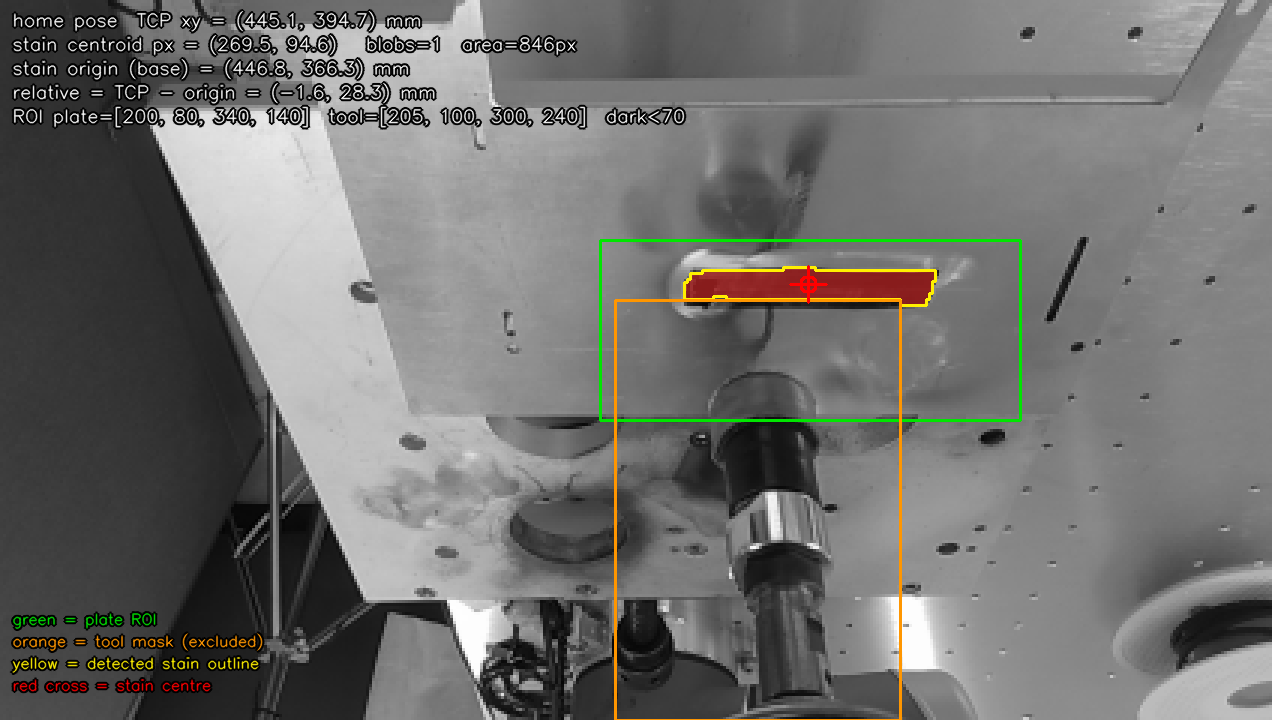
\includegraphics[width=0.87\linewidth]{figures/mark_detection_example.png}
\caption[Marked local region and registration]{Archived camera view of a marked local region and its registration overlay. The colored outlines belong to the existing detection display. This is an example of spatial instruction and image registration, not a validated micro-scratch detector or the fixed-origin E1 trial image.}
\label{fig:mark_example}
\end{figure}

The evaluated E1 comparison fixes \(c=(457.4,375.0)\) mm for all providers. Its evaluation band is specified independently by endpoints and width. The origin is a registration datum; it need not coincide with the midpoint of that band. In E2, the existing per-run origin interface is retained. Neither experiment uses a height-condition label as a policy input.

The policy's external stain-mask option is disabled for the evaluated checkpoints. Instead, the image encoder derives a fixed TCP interaction-region feature from RGB. The physical marking, the registered origin, the evaluator's spatial band, and the encoder's image ROI are therefore four different objects. Conflating them would incorrectly imply that the network is explicitly constrained to the evaluator's band or that it receives a segmentation of the complete processing strategy.

\section{Module Responsibilities}
Figure~\ref{fig:faire_architecture} shows the implemented path from human guidance to evaluation. A provider supplies a sequence, a common execution layer converts it into conditioned commands, and the lower-level controller produces the physical interaction. Measured robot pose and force provide feedback. Evaluation observes this interaction through its own procedural criteria.

\begin{figure}[tbp]\centering
\resizebox{\linewidth}{!}{%
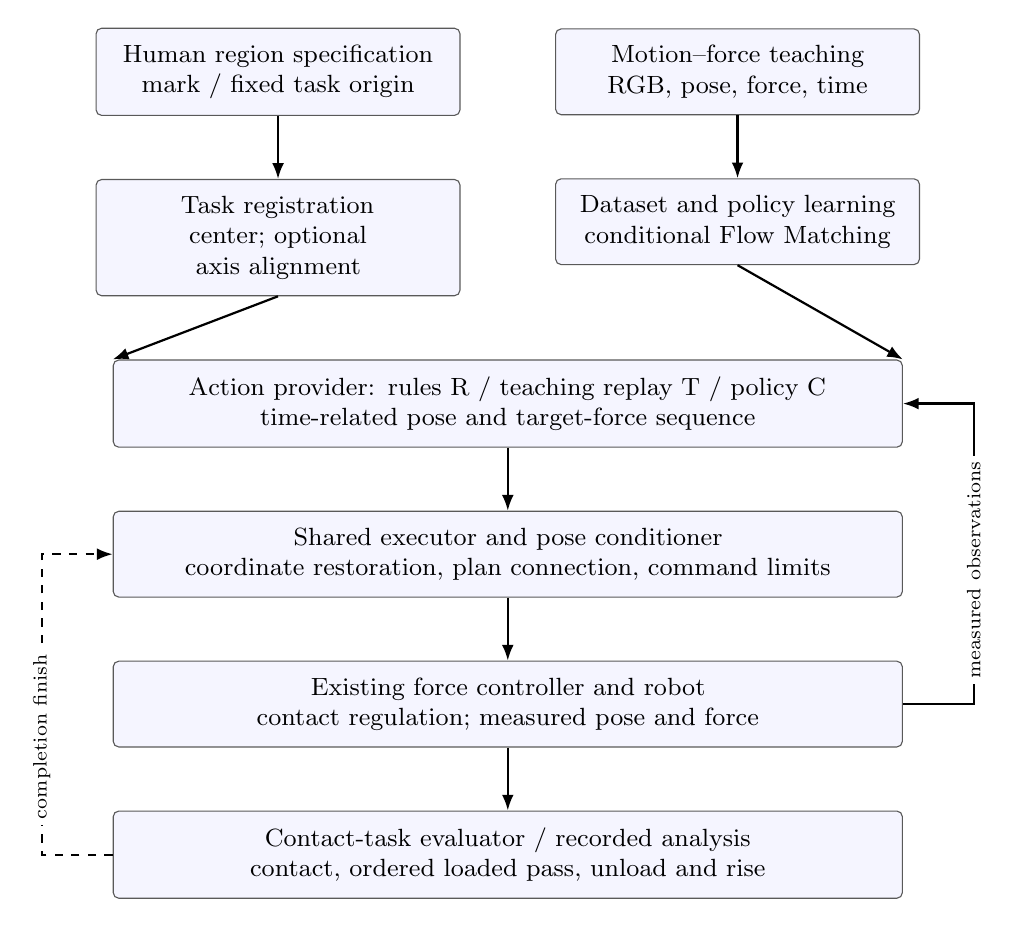
\begin{tikzpicture}[node distance=8mm]
\node[block,text width=42mm] (human) {Human region specification\\mark / fixed task origin};
\node[block,text width=42mm,right=12mm of human] (teach) {Motion--force teaching\\RGB, pose, force, time};
\node[block,text width=42mm,below=of human] (registration) {Task registration\\center; optional axis alignment};
\node[block,text width=42mm,below=of teach] (learning) {Dataset and policy learning\\conditional Flow Matching};
\node[block,text width=96mm,below=10mm of $(registration.south)!0.5!(learning.south)$] (provider) {Action provider: rules R / teaching replay T / policy C\\time-related pose and target-force sequence};
\node[block,text width=96mm,below=of provider] (exec) {Shared executor and pose conditioner\\coordinate restoration, plan connection, command limits};
\node[block,text width=96mm,below=of exec] (control) {Existing force controller and robot\\contact regulation; measured pose and force};
\node[block,text width=96mm,below=of control] (eval) {Contact-task evaluator / recorded analysis\\contact, ordered loaded pass, unload and rise};
\draw[link] (human)--(registration);\draw[link] (teach)--(learning);
\draw[link] (registration.south)--(provider.north west);
\draw[link] (learning.south)--(provider.north east);
\draw[link] (provider)--(exec);\draw[link] (exec)--(control);\draw[link] (control)--(eval);
\draw[link] (control.east)--++(9mm,0)|- (provider.east);
\node[rotate=90,font=\scriptsize,fill=white,inner sep=2pt]
 at ($(control.east)+(9mm,17mm)$) {measured observations};
\draw[link,dashed] (eval.west)--++(-9mm,0)|- (exec.west);
\node[rotate=90,font=\scriptsize,fill=white,inner sep=2pt]
 at ($(eval.west)+(-9mm,15mm)$) {completion finish};
\end{tikzpicture}}
\caption[System overview and module interfaces]{Implemented system overview. Solid arrows show data or execution flow. The dashed arrow requests the existing finish/hold after procedural completion; it does not synthesize an exit motion. The diagram is conceptual and editable. E2 uses its separate operator-terminated protocol.}
\label{fig:faire_architecture}
\end{figure}

\begin{table}[tbp]\centering\small
\caption[Module responsibilities]{Responsibilities of the human and system components.}
\label{tab:module_responsibilities}
\begin{tabularx}{\textwidth}{P{0.24\textwidth}X}
\toprule Component & Responsibility \\ \midrule
Human operator & Specify the local task, demonstrate motion and loading, set up the specimen, and provide recorded field observations. \\
Teaching system & Register tracked tool pose and record paired RGB, pose, force, and receipt-time evidence. \\
Skill provider & Supply a time-related reference sequence using a rule, a fixed demonstration, or a conditioned generator. \\
Common executor & Restore coordinates, interpolate references, connect plans, condition commands, and manage the existing finish/hold procedure. \\
Lower-level controller & Regulate physical contact using the supplied target force and measured state. \\
Task evaluator & Recognize the defined contact procedure and report its outcome; it does not measure surface quality. \\
\bottomrule
\end{tabularx}
\end{table}

\section{Physical Platform and Observations}
The robot interface is the UR10 system identified by the deployed \texttt{ur10skku} topics and Cartesian command services. The teaching side uses a Vive tracker, calibrated tool pose, force/torque sensing, and a RealSense RGB stream. Robot execution records TCP pose from robot feedback and a processed six-axis wrench. The policy uses only the three force components. Torques remain useful logged diagnostics but are not policy inputs or actions for these checkpoints.

\begin{figure}[tbp]\centering
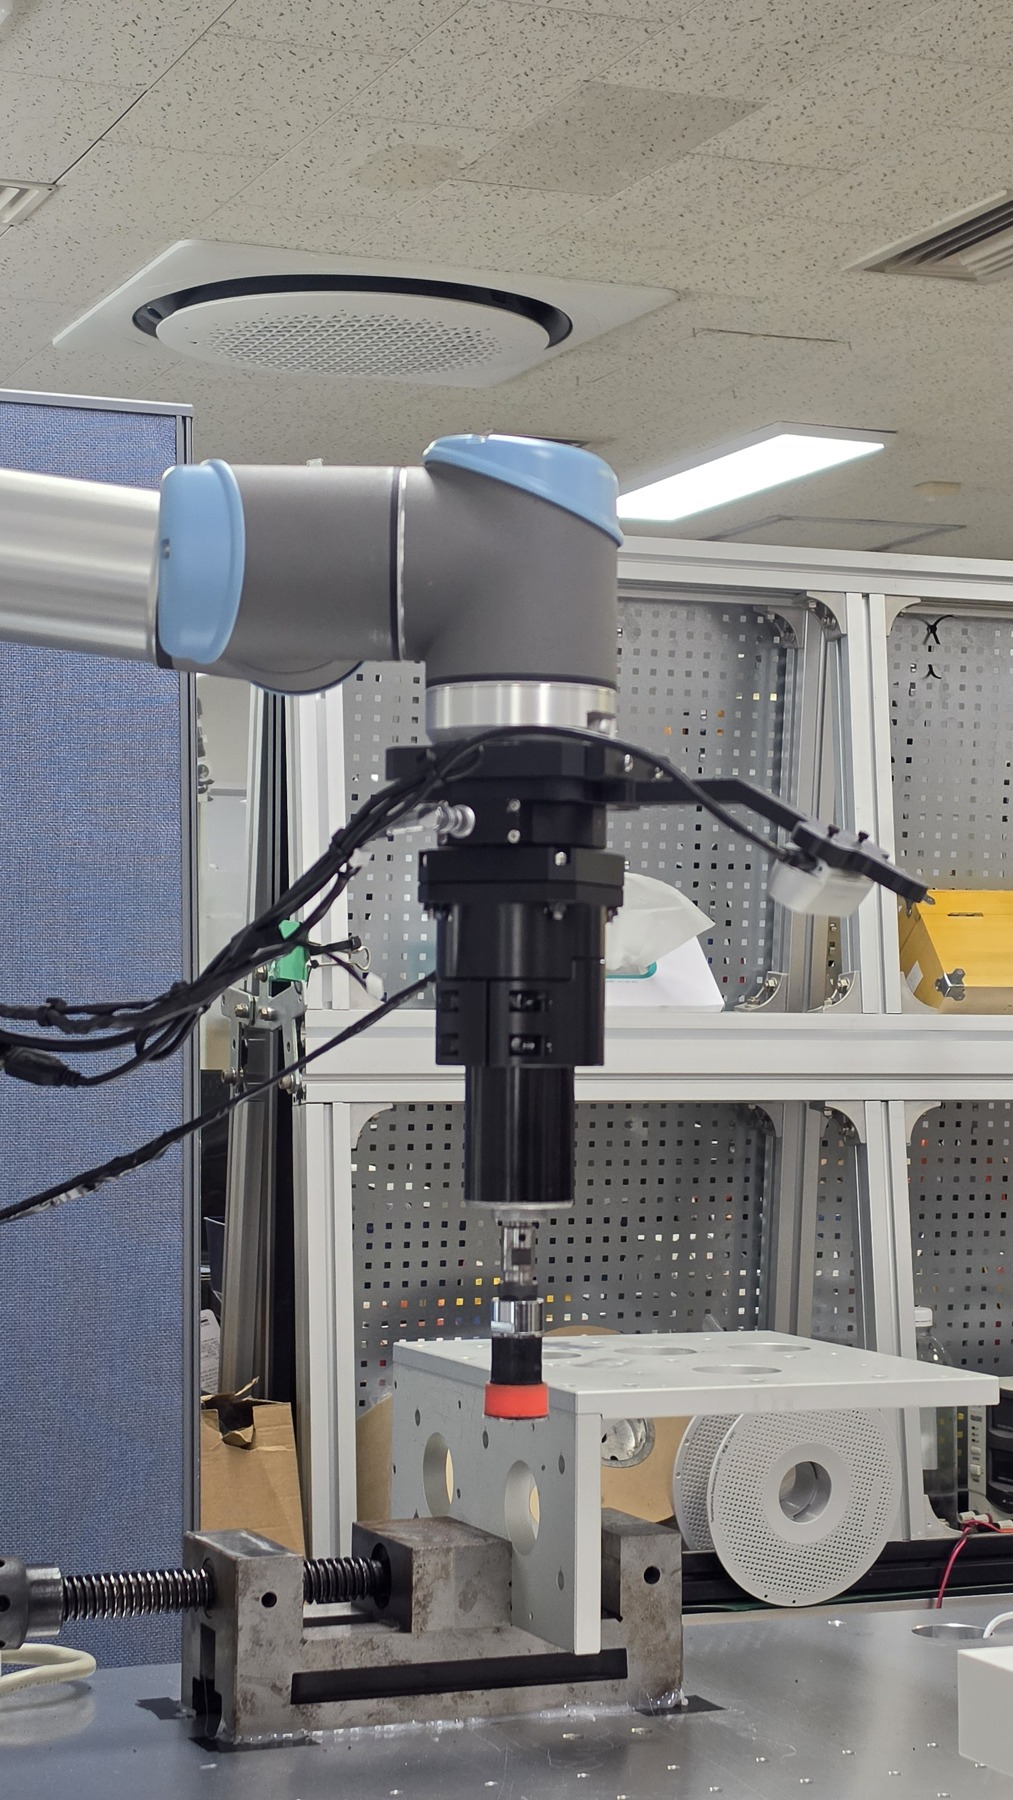
\includegraphics[width=0.67\linewidth,height=0.49\textheight,keepaspectratio]{figures/apparatus_20260807.jpg}
\caption[Archived robot apparatus photograph]{Genuine archived apparatus photograph dated 7 August 2026, showing the robot-mounted processing tool and fixture. Only image rotation and proportional resizing were applied. It illustrates the local experimental platform; it is not presented as a photograph taken during the October E1 or E2 runs.}
\label{fig:apparatus}
\end{figure}

The available records support a description of a robot-mounted local processing tool acting on a marked plate. They do not specify a complete process qualification, including measured spindle speed, material alloy, abrasive grade, or pre/post roughness. The experiments therefore use the measured robot interaction to answer procedural questions. These limits do not prevent reproducing the learning and execution interfaces, but they restrict claims about manufacturing outcomes.

\section{Stain-Centered Learning and Direction Transfer}
\label{sec:stain_relative_generalization}
The representation separates the local movement pattern from its placement on the plate. Its training-data transformation expresses observation and action positions relative to a frozen stain center:
\begin{equation}
 \widetilde p_k=[p_{k,x}-c_x,\ p_{k,y}-c_y,\ p_{k,z}]^\mathsf{T},
 \qquad \widetilde\rho_k=\rho_k.
 \label{eq:relative_task_pose}
\end{equation}
This transformation retains the base-axis orientation and absolute Z coordinate. A single-direction demonstration consequently teaches a center-relative movement pattern in its original reference direction. The implementation additionally supports transferring that learned pattern to another in-plane stain direction through coordinated observation and action transformations. Training on centered positions and aligning directions at inference are two connected parts of the transfer mechanism; the dataset converter itself does not rotate the training episodes.

\subsection{Center and Axis from the Specified Region}
The reference-free registration path detects dark pixels within a configured plate area, excludes the tool area, and maps the retained pixels to robot-base XY coordinates using each image's pose-dependent planar homography. It pools these mapped points across the registration frames. Starting from their coordinate-wise median, four iterations retain the nearest 85\% of points and update the center by their mean. A singular-value decomposition of the trimmed, centered point cloud supplies the dominant strip axis. Its angle \(\theta_{\mathrm{live}}\in[0,\pi)\) is measured in base-plane radians. The axis is unoriented: the same strip has directions differing by \(\pi\), rather than an identified stroke-start endpoint.

The resulting center and optional angle are frozen together for the episode. An operator-supplied live angle is also supported. The direction therefore enters through explicit task registration rather than a learned output head. A center recovered from the visible mark identifies the intended task; it does not estimate defect depth or determine the desired force schedule.

\subsection{Observation Alignment and Path Restoration}
Let \(\theta_{\mathrm{ref}}\) denote the base-plane axis associated with the teaching reference direction. The implemented alignment angle and planar rotation are
\begin{align}
 \alpha&=\operatorname{wrap}_{\pi}
       (\theta_{\mathrm{ref}}-\theta_{\mathrm{live}}),
 &\operatorname{wrap}_{\pi}(\delta)
   &=((\delta+\pi/2)\bmod\pi)-\pi/2,\label{eq:stain_axis_alignment}\\
 R_2(\alpha)&=\begin{bmatrix}
  \cos\alpha&-\sin\alpha\\\sin\alpha&\cos\alpha
 \end{bmatrix}.&&\nonumber
\end{align}
The wrapped angle lies in \([-\pi/2,\pi/2)\). For an absolute measured XY position \(p_{k,xy}\), the policy-side position is
\begin{equation}
 u_k=R_2(\alpha)(p_{k,xy}-c).
 \label{eq:stain_canonical_observation}
\end{equation}
Center subtraction is applied first, followed by alignment to the teaching direction, and then by the checkpoint's numerical normalization. After the policy generates a sequence and the action bounds are inverted, each predicted XY position \(\widehat u_{k+j}\) is restored as
\begin{equation}
 p_{k+j,xy}^{\mathrm{ref}}
   =c+R_2(-\alpha)\widehat u_{k+j}.
 \label{eq:stain_canonical_action}
\end{equation}
The same inverse operation restores the stored demonstration-start XY pose before initial alignment. Thus both the live observation and generated path use the same frozen center and angle. Disabling direction alignment gives \(\alpha=0\) and reduces these equations to the translation-relative path used in E1/E2.

The single-camera policy image can also be rotated in plane about the configured TCP-ROI center, using the alignment angle and a configurable image-coordinate sign. The implementation uses bilinear image interpolation and reflected borders. This operation changes the image supplied to the policy while retaining the original view for recording and display. It adapts the visible direction to the reference view; a planar image rotation does not establish complete perspective or lighting invariance.

Only XY position is rotated by this adapter. Z, tool rotation-vector channels, target-force channels, and measured-force history retain their existing conventions. The method transfers a planar stroke direction while preserving the learned tool-posture and force interfaces; it is not a full rigid-frame transformation of pose and wrench. Its spatial role is distinct from observation-conditioned generation of the local motion--force sequence.

The current launch defaults leave direction alignment disabled. When enabled, the declared reference angle is \(132^\circ\), image rotation is enabled, and the maximum accepted alignment magnitude is \(65^\circ\). These are configurable reference and operating values, not a measured generalization range; the dataset name containing ``90deg'' is not used to infer the base-axis reference angle. If no live angle is available or the configured magnitude is exceeded, the implementation retains translation-only operation. Chapter~\ref{chap:demonstration_collection} distinguishes these implemented transfer operations from the particular dataset and settings used in the measured comparisons.

\section{Supported Conditions and Observable Success}
The E1/E2 datasets and runtime settings use center-relative XY coordinates with direction alignment disabled. Their results assess strategy generation and force-information use within that configuration, rather than supplying a quantitative test of the implemented rotation-transfer mechanism.

E1 defines observable success as contact formation, a continuous loaded ordered traversal of the fixed band, and a simultaneous unloaded upward exit. E2 uses the documented operator-based completion interpretation, corrected for the interrupted A4 attempt. The two definitions serve different recorded protocols and are not pooled into one success statistic.

There is no learned termination output in the evaluated policy. A generated upward movement may reflect the demonstration's temporal structure. Recognition that the procedural exit has occurred belongs to the evaluator in E1 or to the operator's stopping decision in E2. Neither establishes that all defects have been removed. This distinction maintains a clear boundary between the generated skill and the state of the physical surface.

\chapter{Motion--Force Demonstration and Dataset Construction}
\label{chap:demonstration_collection}

\section{Teaching as a Source of Temporal Process Structure}
The purpose of teaching is to supply the motion and loading that remain unspecified by a local region. A demonstration records a tool's approach, motion through the working region, and departure together with the interaction force. This pairing supplies a temporal example for either direct replay or policy supervision. It does not include an independently measured defect-depth trajectory or a label that certifies material-removal completion.

The teaching system combines Vive tracking, a calibrated tool-pose publisher, force/torque sensing, and a RealSense RGB stream. The archived collection interface records six pose components and the first three force components. The paired data used by the evaluated models have a single RGB camera. Figure~\ref{fig:teaching_frames} shows actual frames from the selected replay episode's source, rather than a rendered apparatus or a substitute robot.

\begin{figure}[tbp]\centering
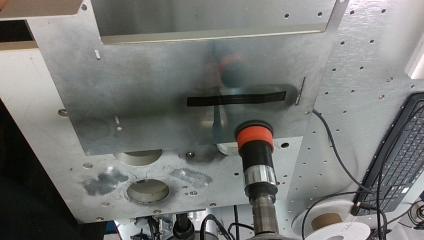
\includegraphics[width=.48\linewidth]{figures/teaching_ep29_frame000.png}\hfill
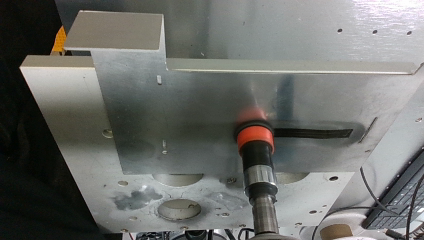
\includegraphics[width=.48\linewidth]{figures/teaching_ep29_frame085.png}\\[3pt]
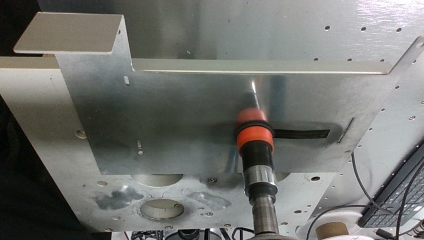
\includegraphics[width=.48\linewidth]{figures/teaching_ep29_frame150.png}\hfill
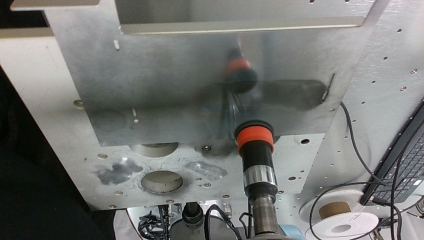
\includegraphics[width=.48\linewidth]{figures/teaching_ep29_frame400.png}
\caption[Actual teaching-camera frames]{Actual teaching-camera RGB frames associated with episode 29 at stored indices 0, 85, 150, and 400. The corresponding source is merged episode \texttt{ep\_0003}, recorded on 19 August 2026. The view shows the tool and marked plate during the recorded operation. It does not show the full tracker or sensor assembly.}
\label{fig:teaching_frames}
\end{figure}

\section{VR Registration and Tracker-to-Tool Conversion}
The recorded pose must refer to the tool rather than the tracker housing. Let \(V\) be the tracking frame, \(T\) the tracked rigid body, \(E\) the tool/TCP frame, and \(B\) the robot base. The nominal rigid coordinate chain is
\begin{equation}
 {}^BT_E(t)={}^BT_V\,{}^VT_T(t)\,{}^TT_E.
 \label{eq:demo_transfer}
\end{equation}
The fixed transforms identify the tracking world with the robot base and remove the tracker-to-tool offset. Translation is expressed in millimeters, while the final orientation is converted to a rotation vector in radians.

The implementation includes more than one rigid transform. Its calibration utilities solve the registration and tool offset, project rotations to valid rotation matrices, and support a planar correction and a bounded XY-dependent position residual. The tracker publisher converts OpenVR translation from meters to millimeters before applying the downstream calibration chain. It right-multiplies the configured spatial-angle alignment and applies the selected tool-offset convention. The published \texttt{calibrated\_pose} is the final tool pose used by the recorder; the raw tracker rotation is not substituted for it in force-axis reconstruction.

The available calibration YAML records a 47-sample fit, planar correction, and a quadratic XY residual. Its stored residual RMS changes from 4.809 to 3.179 mm for that fit. These are calibration-fit diagnostics, not an independent accuracy test of every demonstration or October execution. The source also contains a configurable final constant offset. Consequently, a single conceptual frame-chain diagram is useful for understanding the registration, while the archived parameter file remains necessary for reproducing its numerical convention.

\begin{figure}[tbp]\centering
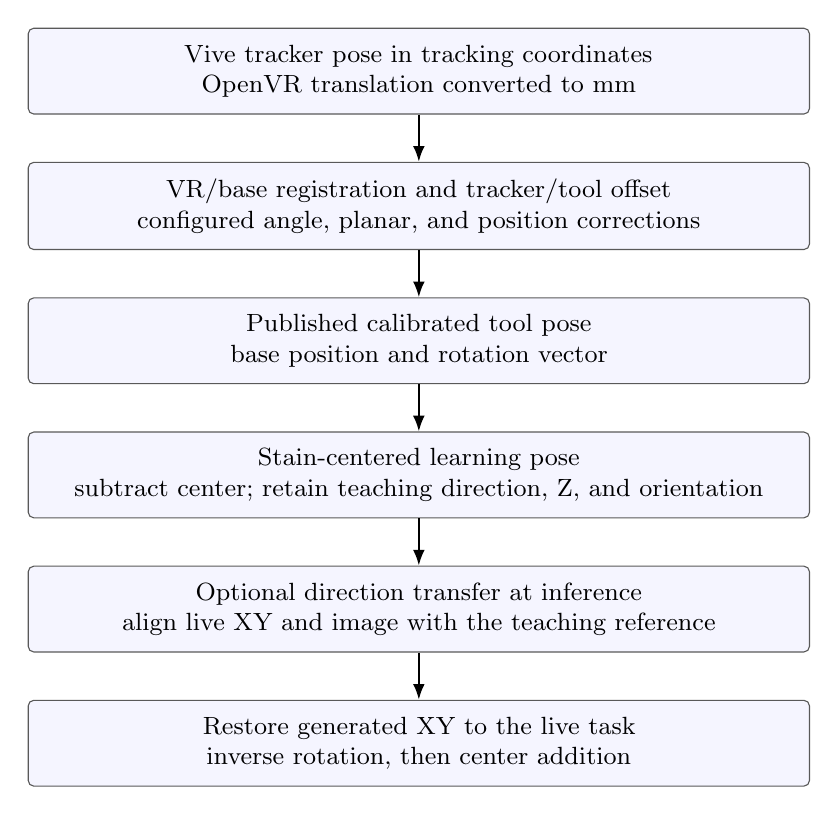
\begin{tikzpicture}[node distance=6mm]
\node[block,text width=95mm] (a) {Vive tracker pose in tracking coordinates\\OpenVR translation converted to mm};
\node[block,text width=95mm,below=of a] (b) {VR/base registration and tracker/tool offset\\configured angle, planar, and position corrections};
\node[block,text width=95mm,below=of b] (c) {Published calibrated tool pose\\base position and rotation vector};
\node[block,text width=95mm,below=of c] (d) {Stain-centered learning pose\\subtract center; retain teaching direction, Z, and orientation};
\node[block,text width=95mm,below=of d] (e) {Optional direction transfer at inference\\align live XY and image with the teaching reference};
\node[block,text width=95mm,below=of e] (f) {Restore generated XY to the live task\\inverse rotation, then center addition};
\draw[link](a)--(b);\draw[link](b)--(c);\draw[link](c)--(d);
\draw[link](d)--(e);\draw[link](e)--(f);
\end{tikzpicture}
\caption[Coordinate-processing and direction-transfer chain]{Implemented coordinate-processing roles, shown as an editable conceptual diagram. Calibration establishes the tool pose; center-relative learning and optional direction alignment register the local movement pattern. The last two boxes show the inference transfer in Equations~\eqref{eq:stain_canonical_observation} and~\eqref{eq:stain_canonical_action}, disabled in E1/E2. Only XY positions are rotated; tool orientation and force channels retain their conventions.}
\label{fig:demo_transfer}
\end{figure}

\section{Synchronized Recording and the Meaning of Time}
The source merged HDF5 identifies its schema as multimodal synchronized recording, its master as camera 0, and its clock as subscriber-receive Unix time. The camera observation supplies the common sample time. Pose and force are associated through receive-time buffers, with a recorded maximum synchronization error parameter of 0.05 s. The archive retains the source times, interpolation indicators, and pose/force synchronization errors for each paired sample.

These timestamps describe software receipt and pairing. They are not hardware exposure timestamps or the original force-sensor acquisition times. Their value is that the construction of a paired sample is explicit and can be inspected. Their limitation is that transport delay and sensor latency cannot be removed simply by assigning all signals to one image time.

The representative source episode records a nominal 30 Hz grid, 443 paired frames, and the original \texttt{sample\_time\_unix} array. The compact learning file retains the paired images and signals but not that full time array. For the replay baseline and the teaching plots, the source episode is recovered using the compact file's \texttt{source\_h5} and \texttt{source\_episode} attributes. This preserves the actual paired time axis instead of reconstructing it solely from the nominal rate.

\section{Signal Stages and Force Processing}
The word raw depends on where a signal enters the pipeline. The recorder's \texttt{raw\_ft} is already a decoded and published measurement after the configured sign, startup-zero, and gravity-processing path. It is raw relative to the recorder's offline filter. It is not an uncorrected packet from the force sensor.

The teaching publisher applies its configured sensor decoding and sign convention, startup mean zeroing, selected publisher filtering, and delta-gravity compensation before publishing the wrench. The recorder then applies native-axis force filtering. In the representative archived episode, the force filter is an exponential moving average with \(\alpha=0.2\),
\begin{equation}
 \bar f_k=\alpha f_k+(1-\alpha)\bar f_{k-1}.
 \label{eq:force_ema}
\end{equation}
The stored pose is processed through the existing Hampel and difference-regularized smoothing pipeline. The archived episode reports no pose EMA, no approach slowdown, and retiming factor one. These are properties of the selected recorded episode; optional processing branches in the current recorder are not assumed to have been active.

\begin{table}[tbp]\centering\small
\caption[Teaching and learning signal stages]{Teaching and learning signal stages. Normalization changes scale for the network; it does not perform physical calibration.}
\label{tab:signal_stages}
\begin{tabularx}{\textwidth}{P{0.25\textwidth}X}
\toprule Stage & Meaning and use \\ \midrule
Published / recorder raw & Decoded and compensated force paired with calibrated pose; preserved as \texttt{raw\_ft} and \texttt{raw\_position}. \\
Filtered recording & Existing pose processing and force EMA; paired images and source-time mapping retained. \\
Learning cleanup & Derived force fields modified by the specified native-axis cleanup; pose and RGB preserved. \\
Normalized tensors & Training-split bounds map pose and force channels to the network scale. B then masks its force-conditioning tensors. \\
\bottomrule
\end{tabularx}
\end{table}

The 12 October force-cleanup dataset is a derived copy. It preserves the 42 episodes' images and pose fields, sets negative native \(F_z\) values to zero, and sets all three force components to zero where the associated stored \(z>175\) mm. Signed \(F_x,F_y\) remain unchanged in the other samples. The same rules apply to observation and action force fields. This height rule is an offline preprocessing convention tied to the stored coordinate system, not a new real-time contact detector or an estimate of material-removal depth.

Figure~\ref{fig:force_processing} shows these stages for the representative episode. Learning nonnegative targets does not impose a nonnegative output constraint on the generator. The archived model checks include negative unconditioned force predictions in some chunks; the runtime must therefore be described from its actual gating and command-processing code, rather than by assuming cleanup enforces a physical output bound.

\figfull{force_processing.pdf}{Actual force-processing stages for teaching episode 29. The upper panel compares post-publisher recorder raw force, offline EMA, and the learning cleanup in native axes. The lower panel rotates the complete cleanup force vector to robot-base axes using its paired tool orientation. These are different signal stages; none is a new physical calibration.}{fig:force_processing}

\section{Force Frames and Common-Axis Analysis}
The existing force correspondence analysis supplies a resolved relation between teaching published axes and the calibrated tool frame:
\begin{equation}
 R_{E\leftarrow\mathrm{pub}}=I,\qquad
 f_B(t)=R_{B\leftarrow E}(t)\,f_{\mathrm{pub,processed}}(t).
 \label{eq:normal_force_projection}
\end{equation}
The second relation is posture dependent. All three force components are rotated using the calibrated tool rotation. Sign, zero, and gravity corrections are already present in the published vector and are not applied again. Translating the XY task origin does not rotate force.

Robot feedback follows a different processing chain: startup zeroing, the archived moving-average stage, a fixed sensor-to-TCP rotation, TCP gravity correction, and TCP-to-base rotation before publication and copying into the current-force topic. The executor's recorded force is therefore already in robot-base axes. Re-rotating that CSV would be incorrect.

Common-axis reconstruction makes the recorded teaching distribution and measured robot-base component comparable for an empirical force-exposure statistic. It does not recover an unlogged controller-applied target or establish a force-tracking error. It also does not imply that training tensors were retrospectively rotated. The evaluated dataset keeps native teaching force, while the inference adapter reads the selected robot-force components directly before normalization. This numerical input convention is retained when reporting the actual evaluated implementation. A common-frame policy-training ablation was not performed.

\section{Relative Coordinates, Episodes, and Data Partitions}
The compact representation subtracts the stored stain center from observation and action XY positions, leaving Z and orientation unchanged. Learning this local pattern removes absolute XY placement from the pose supervision. The selected dataset is labeled single-direction, 90-degree, and explicitly records \texttt{rotation\_aligned=false}. This attribute describes the saved training data; it does not mean that the implementation lacks direction transfer. The separate inference adapter in Section~\ref{sec:stain_relative_generalization} aligns live positions and images to a configured teaching direction and inversely restores generated XY. E1/E2 explicitly disable that adapter, so their results do not quantify its transfer performance. Some upstream files also record episode-specific XYZ corrections, which are preprocessing transformations rather than separate generalization tests.

The evaluated A/B/C models share 42 unique episodes. The optimization partition contains 38 episodes; validation contains episodes 35, 39, 22, and 37. The checkpoint normalizer files reproduce this episode-level partition. All windows from an episode remain in its assigned partition, avoiding overlap of windows from one episode across optimization and validation. This does not establish independence by operator, material, specimen, or collection session. No separate held-out demonstration-test split is claimed.

\figfull{dataset_split.pdf}{Stored lengths of all 42 episodes used by the force-cleanup models. Orange identifies the four validation episodes. The partition is made before window sampling; repeated windows are not independent demonstrations.}{fig:dataset_split}

The loader draws 50 start indices per episode and constructs a 128-step future sequence. End-of-episode padding repeats the final action and masks padded positions out of the loss. Force history includes the current sample and the preceding samples up to a length of 30; a short initial history is padded on the left with the first available value. Start sampling is resampled across training epochs. Its existing phase sampler upweights the one-second precontact period by five relative to free and contact periods, using the recorded force thresholds of 3.0 and 1.2 N. The offline sampler uses this force-derived phase information for all three conditions, including A. A's policy still receives no force observation or force target.

Normalization bounds are computed from optimization-training episodes only. For channel \(d\), the implemented min--max mapping is
\begin{equation}
 \mathcal N_d(x)=2\frac{x-m_d}{\max(M_d-m_d,\epsilon)}-1,
 \label{eq:minmax_normalization}
\end{equation}
where \(m_d,M_d\) are the stored training bounds and \(\epsilon\) is the numerical denominator floor. State and action bounds are stored separately; force history uses the state-force bounds. Normalization does not force all future online values to lie within the training range.

\section{A Representative Motion--Force Pairing}
Episode 29 is used to explain the temporal representation because it is the operator-selected replay source, rather than an episode chosen for low error. Figure~\ref{fig:teaching_motion_force} presents its actual position and force history. The transition from approach to loaded movement and then rising motion gives a structured association between location, loading, and time. Replay uses that association directly; learning uses many such future windows as supervision.

\figfull{teaching_motion_force.pdf}{Teaching episode 29 on the original paired source-time axis. XY is task relative, Z remains in the stored absolute convention, and force is the native-axis cleanup signal. The 175 mm line is the offline cleanup boundary. The curves are not a desired-versus-measured robot force-tracking comparison.}{fig:teaching_motion_force}

The force action derives from measured teaching interaction, not an independently recorded human command. Physical equivalence must be assessed from robot measurements because the mechanics and controller differ.

\chapter{Force-Conditioned Motion--Force Skill Learning}
\label{chap:force_il}

\section{Learning Objective and Observation Interface}
The learning problem is to generate a future local skill from the execution context, while preserving a joint representation of movement and target loading. A conditioned sequence can change at a later inference call when the robot reaches a different pose or contact state. The policy is not asked to estimate scratch depth, choose an abrasive, or output a separate completion decision.

For the force-observing model, the physical observation at index \(k\) is
\begin{equation}
 o_k=\left(I_k,\widetilde q_k,f_k^{\mathrm{meas}},
       f_{k-L+1:k}^{\mathrm{meas}}\right),\qquad L=30.
 \label{eq:il_observation}
\end{equation}
The numerical state has nine components: six Cartesian pose values and three current force values. History has shape \(30\times3\). Only \(F_x,F_y,F_z\) enter this observation; the sensor's torque channels do not. The input image is the single \(240\times424\) RGB view. Images are converted to floating-point tensors and normalized using the implemented RGB channel means and standard deviations.

The action target is a normalized \(128\times9\) sequence of task-relative position, rotation vector, and teaching-derived target force. Position and orientation describe the tool reference, whereas force describes a controller-level target. Both appear in the same sequence so that their temporal correspondence can be learned. The action horizon corresponds to approximately 4.27 s on the nominal 30 Hz action grid. Its last sample is at \(127/30\) s relative to the first, which distinguishes a sample count from an endpoint-to-endpoint duration.

\section{Implemented Observation Encoder}
The active model is the Flow RGB policy in the archived training snapshot. It uses a frozen DINOv3 ViT-small patch-16 image backbone, a state MLP, a one-layer force-history GRU, and a fusion MLP. The separate encoder modules available elsewhere in the repository do not determine this checkpoint's architecture.

The visual branch combines the global image feature with a feature pooled from a fixed TCP interaction ROI. The ROI is constructed internally from reference image dimensions \(424\times240\), center \((253,120)\), and area-fraction parameter 0.25. The DINO patch features in that ROI are pooled by the configured attention mechanism. Global and ROI features are each projected to 512 components. The ROI is a calibrated interaction-region prior, not an external defect mask and not a prediction of surface damage.

The state MLP encodes all nine normalized state components into 256 components. A GRU with input dimension three and hidden dimension 64 encodes the force history, with its final hidden state contributing to fusion. The fused condition is 256-dimensional. Thus the current force appears both in the state vector and as the last history sample. There is no learned moment-history branch, LSTM comparison, or termination head in the evaluated configuration.

\begin{figure}[tbp]\centering
\resizebox{\linewidth}{!}{%
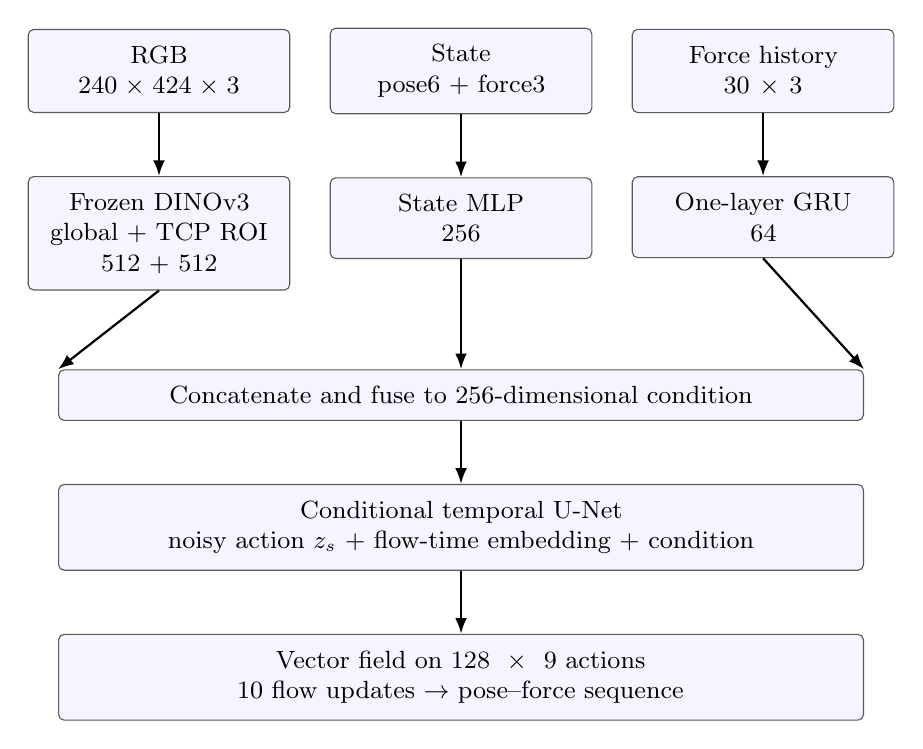
\begin{tikzpicture}[node distance=8mm]
\node[block,text width=29mm] (rgb) {RGB\\$240\times424\times3$};
\node[block,text width=29mm,right=5mm of rgb] (state) {State\\pose6 + force3};
\node[block,text width=29mm,right=5mm of state] (history) {Force history\\$30\times3$};
\node[block,text width=29mm,below=of rgb] (visual) {Frozen DINOv3\\global + TCP ROI\\$512+512$};
\node[block,text width=29mm,below=of state] (mlp) {State MLP\\256};
\node[block,text width=29mm,below=of history] (gru) {One-layer GRU\\64};
\node[block,text width=98mm,below=14mm of mlp] (fuse) {Concatenate and fuse to 256-dimensional condition};
\node[block,text width=98mm,below=of fuse] (unet) {Conditional temporal U-Net\\noisy action $z_s$ + flow-time embedding + condition};
\node[block,text width=98mm,below=of unet] (out) {Vector field on $128\times9$ actions\\10 flow updates $\rightarrow$ pose--force sequence};
\draw[link](rgb)--(visual);\draw[link](state)--(mlp);\draw[link](history)--(gru);
\draw[link](visual.south)--(fuse.north west);\draw[link](mlp)--(fuse);\draw[link](gru.south)--(fuse.north east);
\draw[link](fuse)--(unet);\draw[link](unet)--(out);
\end{tikzpicture}}
\caption[Implemented policy architecture]{Actual force-observing policy configuration, shown conceptually. In B, the current-force and history tensors are zeroed after normalization while the history branch remains. A uses pose6 state/action and omits force history. The flow vector field has the same sequence shape as its action input.}
\label{fig:force_history_policy}
\end{figure}

\begin{table}[tbp]\centering\small
\caption[Architecture and training settings]{Architecture and training settings for the force-cleanup checkpoints used in E1/E2.}
\label{tab:learning_settings}
\begin{tabularx}{\textwidth}{P{0.48\textwidth}X}
\toprule Item & Stored value \\ \midrule
Backbone / trainable status & DINOv3 ViT-small, patch 16 / frozen \\
State / history / global condition & 256 / 64 / 256 components \\
Temporal U-Net channel widths & 256, 512, 1024 \\
Convolution kernel / groups & 5 / 8 \\
Flow-time embedding & 256 components \\
Action horizon / force-history length & 128 / 30 samples \\
Loss / flow integration updates & Masked MSE / 10 \\
Optimizer & AdamW, learning rate \(10^{-4}\) \\
Weight decay / optimizer betas & \(10^{-5}\) / \((0.95,0.999)\) \\
Batch size / training seed & 12 / 0 \\
Training epochs / warmup & 500 / 10 epochs \\
Learning-rate schedule & Cosine; minimum \(10^{-6}\) \\
Gradient norm clip & 1.0 \\
\bottomrule
\end{tabularx}
\end{table}

\section{Flow Matching Sample Construction}
Flow Matching learns a field that transports a simple noise distribution toward the demonstrated sequence distribution~\cite{lipman2023flow}. The following equations describe the particular implemented construction, rather than all possible flow-matching paths.

Let \(A\in\R^{H\times d_a}\) be a demonstrated action chunk after action normalization, with \(d_a=9\) for B/C and \(d_a=6\) for A. Independently sample a noise chunk \(Z_0\sim\mathcal N(0,I)\) with the same shape and a scalar flow time
\begin{equation}
 s\sim\mathcal U(\varepsilon,1-\varepsilon),\qquad\varepsilon=10^{-4}.
\end{equation}
The source implementation uses
\begin{equation}
 Z_s=(1-s)Z_0+sA,\qquad U=A-Z_0.
 \label{eq:flow_training_path}
\end{equation}
The vector-field network \(v_\theta(Z_s,s,c_k)\) predicts \(U\), conditioned on the encoded observation \(c_k=E_\theta(o_k)\). The scalar \(s\) belongs to a dimensionless generative process. It is unrelated to the physical polishing time \(t\) or the future sample index \(j\).

Let \(m_j\) equal one when future step \(j\) has actual episode support and zero when it is padded. The implemented per-batch objective is
\begin{equation}
 \mathcal L_{\mathrm{FM}}=
 \frac{\displaystyle\sum_{b,j,d}m_{bj}
 \left[v_\theta(Z_{s_b},s_b,c_b)_{jd}-(A_b-Z_{0,b})_{jd}\right]^2}
 {d_a\,\max\!\left(1,\sum_{b,j}m_{bj}\right)}.
 \label{eq:imitation_loss}
\end{equation}
Here \(b\) indexes batch elements, \(j\) future action steps, and \(d\) action coordinates. A new noise tensor and flow time are sampled for the training evaluation. All valid normalized coordinates contribute to the same MSE. There are no additional orientation-geodesic, target-force-tracking, material-removal, or completion losses in this configuration.

The conditional temporal U-Net operates along the action-sequence dimension. Its residual blocks combine temporal convolutions with the global observation and flow-time condition. The configured channel levels are 256, 512, and 1024; convolutional blocks use GroupNorm and Mish nonlinearities. These choices parameterize the field rather than creating a separate head for each physical objective. In particular, a lower force-related loss is not computed independently from the motion coordinates.

\section{Flow Integration and Physical Timing}
At inference, a fresh Gaussian chunk \(Z^{(0)}\) is generated. With \(M=10\) and \(h=1/M\), the source applies
\begin{equation}
 Z^{(m+1)}=Z^{(m)}+h\,
 v_\theta\!\left(Z^{(m)},(m+\tfrac12)h,c_k\right),
 \quad m=0,\ldots,M-1.
 \label{eq:flow_integration}
\end{equation}
This is the exact explicit update with a midpoint flow-time argument used in the code. It is not a two-stage midpoint Runge--Kutta solver: no intermediate state evaluation is computed. The final sequence is denormalized using the stored action bounds, and its relative XY coordinates are restored before execution. When the implemented direction-transfer option is active, observation XY and the single-camera policy image are aligned before conditioning, and generated XY is inversely rotated before center addition, as defined in Section~\ref{sec:stain_relative_generalization}. This adapter surrounds the learned generator without changing its training objective or adding a predicted direction channel. It is disabled in the evaluated E1/E2 runs.

Ten flow updates generate an entire chunk. They are not ten physical polishing steps, and the physical action grid does not run at the flow-integration frequency. Online generation is triggered through a 5 Hz inference timer but is gated by existing plan age: the nominal stride is 120 samples at 30 Hz, or four seconds of reference progression. The actual recorded calls are separated by timer scheduling and inference latency as well. This gives observation-conditioned replanning at chunk boundaries, not a claim of continuous high-frequency strategy correction.

The force history also has two time interpretations. In the dataset, 30 samples on a nominal 30 Hz grid describe approximately one second of historical context. Online, the adapter retains the most recent 30 force callback values and left-pads an insufficient history; it does not resample them onto an exact one-second clock. A 20 Hz recording cap for diagnostic CSV files does not specify the policy callback rate. The history length is therefore reported as a sample count, with its nominal training duration stated separately.

\section{Separating Force Output from Force Observation}
The three E2 conditions implement different information contracts. A has a six-dimensional pose state and six-dimensional pose action, with no force-history encoder or force supervision. An external constant target is supplied by the execution interface. B retains the nine-dimensional action and the same history architecture as C, but the current-force part of its normalized state and its normalized history tensor are replaced by zeros. C retains the measured-force inputs.

Masking occurs in the dataset/model conditioning path during training and again at the inference boundary. It does not alter the force-action target. Because masking is applied after normalization, a zero conditioning value is a neutral network input, not a declaration that physical measured force is zero newtons. B remains a separately trained model, rather than C evaluated with a missing input it was never trained to receive.

The force signal is still used by the common executor and lower-level controller in A and B. It is also used by the existing offline phase sampler. Thus ``force observation OFF'' refers specifically to the policy's conditioning channels. Chapter~\ref{chap:experiments} uses this distinction to interpret the A/B comparison as a force-output comparison and B/C as a force-observation comparison, subject to the limitations of separate single-seed training.

\section{Training Completion and Checkpoint Selection}
The recorded training completed 500 epochs per condition, ending at zero-based epoch 499. The deployed best checkpoints are selected by minimum validation loss, as confirmed by both the model manifest and the checkpoint metadata. Table~\ref{tab:checkpoints} distinguishes the configured duration from the selected epoch.

\begin{table}[tbp]\centering\small
\caption[Selected checkpoint epochs]{Selected checkpoints. Epoch values follow the stored zero-based convention. Validation losses have different action dimensions for A versus B/C and are not task-performance scores.}
\label{tab:checkpoints}
\begin{tabular}{lrrrr}
\toprule Model & State/action dim. & Best epoch & Final epoch & Best val. loss \\ \midrule
A & 6 / 6 & 39 & 499 & 0.049722 \\
B & 9 / 9 & 42 & 499 & 0.069948 \\
C & 9 / 9 & 42 & 499 & 0.066444 \\
\bottomrule
\end{tabular}
\end{table}

Validation evaluates the same flow-field objective using held-out episodes. Its minimum selects a generative model according to that objective, not according to robot task completion or measured finish quality. Since noise and flow time enter the loss evaluation, the numerical minimum also should not be interpreted as a deterministic physical optimum. There is one recorded training seed per condition. Five robot repetitions per condition evaluate execution of that trained model; they do not constitute five independently trained policies.

The resulting method offers a concrete mechanism for coupling motion and target loading under observations. Whether the mechanism improves a given local task remains an empirical question. Its demonstrated function is generation and deployment of the specified action representation; its broader value is assessed alongside rules and replay in the following chapters.

\chapter{Robot Execution and Contact-Task Evaluation}
\label{chap:execution}

\section{From a Skill Sequence to Robot Commands}
The generated sequence is an upper-level reference. Its physical meaning depends on the execution system that samples it, connects new plans, gates force, and transmits commands to the existing controller. A common execution layer is therefore necessary for interpreting differences between providers.

The provider interface supplies a time array, pose--force values, a plan identifier, and whether the plan is finite. R supplies a prescribed finite path with a recipe force. T supplies a finite teaching sequence with its original time axis. C supplies successively generated chunks from observations. Relative XY positions are restored using the frozen task origin before commands are interpreted in robot-base position coordinates. In the optional direction-transfer path, inverse XY rotation precedes that addition; the evaluated E1/E2 configuration uses translation alone. This restoration occurs before downstream command conditioning. The accompanying force values remain controller targets, with their frame interpreted by the lower-level configuration.

The timed sampler uses elapsed reference time rather than selecting the closest spatial waypoint. It linearly interpolates position and force and interpolates orientation on \(SO(3)\). This preserves the association between a source time and its requested pose/force. It does not guarantee identical physical feed velocity, because downstream conditioning and contact dynamics can alter motion.

\section{Shared Pose Conditioning and Plan Connection}
The evaluated E1 configuration applies the same archived pose conditioner to R, T, and C. Earlier metadata within the profile still refers to its initial C-only introduction; the active shared R/T/C wrapper and recorded runtime establish the later comparison's actual scope. R/T are presented through a private 30 Hz, 128-point pose view with a 120-point stride, while their original finite force/time plans remain the source for force sampling and phase boundaries.

The conditioner smooths XYZ with a 35-point moving average and orientation with a quaternion mean. The latter avoids averaging rotation vectors through their branch cut near \(\pi\). Edge padding is confined to the filter's window construction. A replacement plan is joined to the preceding reference and velocity over 0.5 s. Its quintic connection weight is
\begin{equation}
 \beta(u)=10u^3-15u^4+6u^5,\qquad
 u=\min(1,(t-t_b)/0.5),
 \label{eq:plan_connection}
\end{equation}
where \(t_b\) is the connection start. Position connects from a velocity-extended anchor; orientation uses a bounded relative rotation. The conditioner also retains its velocity state across replacement plans and bounds the change in commanded velocity.

These operations alter the reference actually presented to the command loop. They are shared processing choices, rather than evidence that the generated raw chunks are intrinsically smooth. Likewise, T's time scaling of one describes its source-time replay, not equality between the demonstrator's and robot's measured instantaneous speed.

\begin{figure}[tbp]\centering
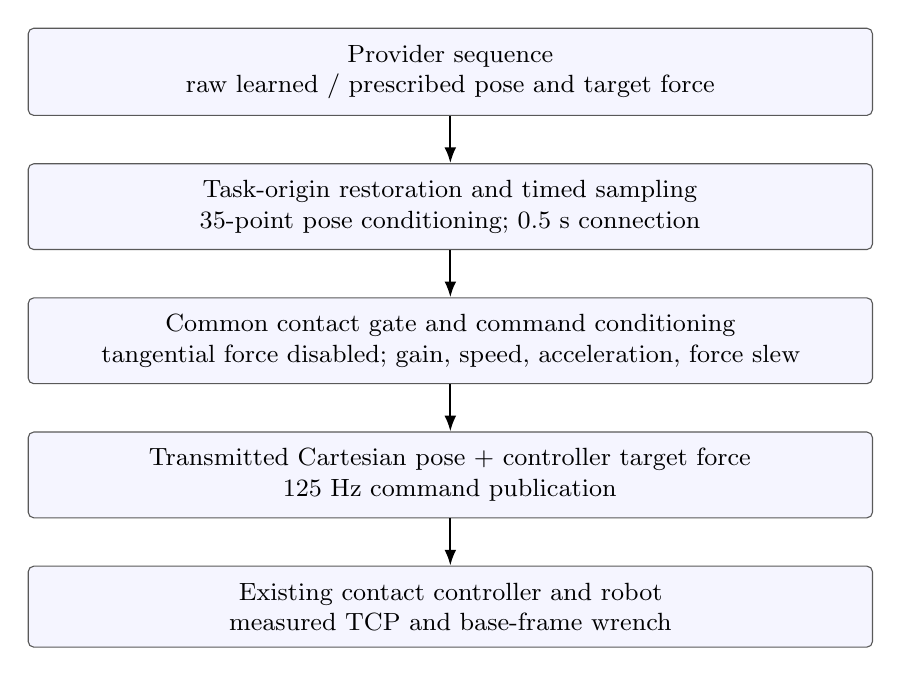
\begin{tikzpicture}[node distance=6mm]
\node[block,text width=103mm] (p) {Provider sequence\\raw learned / prescribed pose and target force};
\node[block,text width=103mm,below=of p] (c) {Task-origin restoration and timed sampling\\35-point pose conditioning; 0.5 s connection};
\node[block,text width=103mm,below=of c] (g) {Common contact gate and command conditioning\\tangential force disabled; gain, speed, acceleration, force slew};
\node[block,text width=103mm,below=of g] (s) {Transmitted Cartesian pose + controller target force\\125 Hz command publication};
\node[block,text width=103mm,below=of s] (l) {Existing contact controller and robot\\measured TCP and base-frame wrench};
\draw[link](p)--(c);\draw[link](c)--(g);\draw[link](g)--(s);\draw[link](s)--(l);
\end{tikzpicture}
\caption[Command processing and contact execution]{Execution interface and distinct command stages. The transmitted target is observable in executor logs; the controller-applied target is not available as a synchronized time series. This conceptual diagram describes command processing, not measured force-tracking performance.}
\label{fig:execution_architecture}
\end{figure}

\section{Command Rates, Limits, and Force Gating}
The command loop uses a nominal 0.008 s period, corresponding to 125 Hz. The common proportional command-update gain is 15 s\(^{-1}\), with per-axis position speed cap 10 mm/s and angular cap 40 degrees/s. The pose-conditioning acceleration settings are 25 mm/s\(^2\) and 100 degrees/s\(^2\). The force-command slew limit is 30 N/s. These are command-processing settings, not experimentally measured limits of physical tool speed or contact force.

For a scalar translational component, the shared update can be represented as
\begin{equation}
 \delta x_i=\operatorname{clip}\bigl(\min(1,K\Delta t)(x_i^\star-x_i^{\mathrm{cmd}}),
                    -v_i^{\max}\Delta t,v_i^{\max}\Delta t\bigr),
 \label{eq:command_update}
\end{equation}
followed by the existing acceleration conditioning. \(x_i^\star\) is the sampled conditioned reference, \(K=15\) s\(^{-1}\), and \(\Delta t\) is bounded by the nominal control period. Orientation uses a relative-rotation increment instead of direct component-wise interpolation across a branch cut.

The operational gate reads measured robot-base \(F_z^B\), enters contact at 3.0 N, and leaves at 1.2 N. While the gate is OFF, the requested normal target is suppressed. The command's tangential force components are set to zero in the evaluated common executor. Thus B/C learn a three-component force action, but the deployed comparison transmits only its normal-force component as a nonzero target. Their three-component measured-force observations can still inform generation.

The target's final approach to its requested value is affected by gain and slew conditioning. A nominal constant recipe is therefore distinct from the full transmitted force curve, particularly around contact onset and release. In E1, R uses 18 N. In E2, A uses an external 23 N target. The operator's approximate 20 N teaching intention, those recipe values, and the measured base-force distribution describe different quantities.

\section{Existing Lower-Level Contact Regulation}
The archived controller receives a Cartesian pose reference and a signed target-force vector. Its TCP-coordinate path rotates measured base vectors into the local frame, performs contact-control computation there, and restores the resulting motion to the robot frame. The stored controller configuration identifies TCP force coordinates and an existing mass/damping adaptation mode. This lower-level adaptation is a shared control asset; it is not the upper-level residual surface-repair policy proposed in the old thesis.

The underlying admittance implementation defines position error \(e=x_d-x_c\) and force error \(F_d-F_{\mathrm{ext}}\). Its scalar virtual dynamics can be written as
\begin{equation}
 M\ddot e+D\dot e+Ke=F_d-F_{\mathrm{ext}},\qquad x_c=x_d-e,
 \label{eq:admittance_il}
\end{equation}
where \(x_d\) is the supplied motion reference, \(x_c\) the compliant motion output, and \(M,D,K\) the virtual mass, damping, and stiffness. This controller calculation converts position to meters internally; its translational parameter units are kg, N\,s/m, and N/m. The source discretizes the relation using the Tustin form and contains mode-dependent parameter updates. Equation~\eqref{eq:admittance_il} explains the interaction role; it does not replace the deployed switching and adaptation logic with a newly designed controller.

Teaching force, policy output, transmitted target, and measured force must remain distinct. The available axis correspondence permits rotating teaching measurements into robot-base coordinates for analysis. It does not provide the actual controller-applied reference after all internal processing. For that reason, the thesis does not subtract published TCP target \(F_z\) directly from measured base \(F_z\) and call the result tracking RMSE.

\section{Approach and Contact-Start Synchronization}
R and T retain an existing one-time contact-start synchronization. Before confirmed contact, their approach reference continues to progress up to the prescribed processing boundary. Once distinct received force observations sustain the existing ON state for 0.2 s, the reference clock is aligned to that boundary. After the alignment, the finite strategy advances from its source timing; repeated synchronization is not applied.

This mechanism matters because the physical surface can be encountered before or after a nominal geometric boundary. It supplies feedback to fixed strategies without learning a policy. C instead generates its own approach and later chunks from observations. Common contact gating and lower-level force regulation remain active in all methods.

The normal departure is also provider dependent. R includes a planned zero-force upward segment, T contains the selected teaching exit, and C can generate an exit within its pose--force sequence. The evaluator recognizes the result of these actions. It does not insert a new retraction to make a deficient sequence satisfy the task.

\section{The Executed E1 Contact Procedure}
E1 uses a fixed 25 mm-wide XY band between \(P_0=(445,395)\) mm and \(P_1=(487,345)\) mm. Its length is 65.299 mm and it is divided into 14 longitudinal segments. The band concerns the TCP center; it is not a measurement of the contact footprint.

Let \(d=(P_1-P_0)/\ell\), \(\ell=\|P_1-P_0\|\), and let \(n\) be a unit vector perpendicular to \(d\) in the XY plane. For TCP XY position \(p_{xy}\), define longitudinal and transverse coordinates
\begin{equation}
 u=d^\mathsf{T}(p_{xy}-P_0),\qquad
 v=n^\mathsf{T}(p_{xy}-P_0).
 \label{eq:task_band}
\end{equation}
Band occupancy requires \(0\leq u\leq\ell\) and \(|v|\leq12.5\) mm. An ordered loaded candidate starts at an end segment and advances through adjacent first visits toward the opposite end. Contact OFF, missing support, or leaving the band breaks a candidate. Revisiting a previously visited segment does not create additional forward progress. Completion of the 14-segment sequence establishes the required pass. There is no per-segment 0.466 s dwell requirement in this primary criterion.

The executed evaluator first confirms contact for 0.2 s. Its original height reference \(z_{\mathrm{contact}}\) is a time-weighted median over the initial contact-confirmation support. After the required pass, it requires both the OFF state and
\begin{equation}
 z(t)\geq z_{\mathrm{contact}}+5\ \mathrm{mm}
 \label{eq:original_release}
\end{equation}
continuously for 0.2 s. Contact formation, ordered loaded pass, and this exit conjunction define \texttt{TASK\_COMPLETED}. A higher initial reference can prevent the last conjunction even when the subsequent trace shows unloading and a rise from the working surface.

The prepared \texttt{pass\_height\_ref\_v2} changes the reference to the time-weighted median measured Z of the first successful loaded pass. It freezes the reference when that pass completes and retains the same 5 mm rise and simultaneous OFF confirmation. This is a separate evaluation version. Its height-only replay on old records and its unexecuted revised-observer sessions are reported separately in Chapter~\ref{chap:experiments}.

\section{Completion, Observation Support, and Time Windows}
The online evaluator used for the recorded E1 cohort consumes the bracketed recorded pose and force observations. Force is held by zero-order hold (ZOH) and position is interpolated within recorded support; gaps longer than 0.2 s are treated as unobserved. The final offline replay can use a bracket already recorded before stopping that was not yet available when an online decision was made. It does not manufacture 125 Hz sensor samples from the command loop's cached state.

In the prepared revised observer, distinct receipt events and consumed intervals are recorded explicitly. That change improves reproducibility of the online observation stream but cannot reconstruct events that were never logged in the older cohort. It remains separate from the height-only sensitivity analysis.

The primary completion time is the first procedural-completion time measured from execution start. Incomplete attempts have no completion time. The E1 force-analysis window begins at execution start and ends at first completion, or at the first stop if the procedure is incomplete. Subsequent return or hold is excluded. The same window rule is applied to every provider.

Within this window, excess-force exposure is
\begin{equation}
 J_{\mathrm{excess}}=\int_{t_0}^{t_1}
 \max\!\left(F_z^B(t)-Q_{95},0\right)\,dt,
 \qquad Q_{95}=30.812396273\ \mathrm{N}.
 \label{eq:excess_force}
\end{equation}
The reference is the existing episode-balanced, actual-time-weighted teaching cleanup distribution rotated to base axes, with the archived stored-Z candidate convention. It includes validation episodes because it describes the common teaching reference, not a fitted policy input. It is an empirical analysis upper reference, not a damage, safety, or effective-polishing limit. The lower quantile, approximately 0.4498 N, is not used as a contact threshold. Low or zero native-force samples can have nonzero projected base components and do not establish meaningful contact.

E2 has a different stopping protocol: the recorded window ends at the first operator finish request. A terminal software event labeled normal completion verifies the existing stop path rather than task achievement. A4 demonstrates why the two must be separated. The first request time is retained even when the later operator report identifies the task as incomplete.

\section{Execution Timing and Checks}
The action grid (30 Hz), inference timer (5 Hz), plan stride (about 4 s), command publication (125 Hz), and recorded feedback (about 18 Hz) describe different mechanisms. Receipt timestamps and a 20 Hz CSV cap do not identify sensor acquisition or physical response. Existing timing, freshness, workspace, and stop/hold checks remain common infrastructure.

\chapter{Experimental Evaluation}
\label{chap:experiments}

\section{Evaluation Questions and Recorded Cohorts}
The experiments examine the execution value of a local motion--force skill at two levels. E1 varies how the strategy is supplied while retaining the common contact-control environment. E2 varies force output learning and policy force observation. These comparisons address different questions, even though they use the same family of force-cleanup checkpoints.

The primary E1 cohort is the nominal development session recorded on 14 October 2026. It contains five started executions each of R, T, and C. Its frozen configuration version is \texttt{e1ct\_61a19f7d7337a82c}. The actual started order is R, then T, then C. An earlier R5 registration did not reach execution start; the later R5 retry supplies the fifth started R trial. That original non-start remains a separate record in Appendix~\ref{app:runs}. Thus there are 15 measured executions and one additional non-started registration, rather than an implicit deletion of an unsuccessful robot trajectory.

E2 is the 13 October force-cleanup session, with five attempts each of A, B, and C. Its actual execution order is A, then B, then C, regardless of a different order in the preparation notes. All 15 are retained. The A4 task outcome uses the operator's later, explicit field correction: it did not transition to contact release and was stopped while maintaining contact. The original event labels and request timestamps are preserved.

The two C groups are not combined. Nor are the older September or pre-cleanup records combined with the October results. The analysis is descriptive: one trained seed per learned condition and five physical repetitions do not establish population-level reliability or statistical significance.

\section{Platform, Surface, and Experimental Controls}
The local task uses the UR10 platform, the robot-mounted processing tool, and a marked plate visible in RGB. The common execution settings are those in Chapter~\ref{chap:execution}. The task is to approach, process the local region under load, and unload with an upward exit. The mark provides visible task context, while measured TCP pose and base-frame wrench provide the quantitative execution signals.

The records do not supply independent measurements of abrasive state, actual spindle RPM, specimen alloy, scratch depth, mass loss, or roughness change. The archived procedure asks the operator to maintain the same setup within a comparison, but this is not a measurement of identical physical conditions. Ordered collection also allows tool wear, mark preparation, or operator familiarity to vary with method. These factors are considered when interpreting the results.

\begin{table}[tbp]\centering\small
\caption[E1/E2 comparison conditions]{Complementary comparisons. Every condition retains common lower-level force feedback and its experiment's shared command-processing configuration.}
\label{tab:expert_il_baselines}
\begin{tabularx}{\textwidth}{P{0.13\textwidth}p{0.16\textwidth}X}
\toprule Study & Condition & Strategy and force interface \\ \midrule
E1 & R & Rule path, 18 N recipe, existing contact-start synchronization. \\
 & T & Cleanup episode 29 pose/force/time replay, scaling 1.0, existing contact-start synchronization. \\
 & C & Conditioned Flow pose--force chunks with measured-force observation. \\
\midrule
E2 & A & Learned pose only; no policy force observation/history; external 23 N target. \\
 & B & Learned pose and force; current-force and history conditioning zeroed. \\
 & C & Learned pose and force; measured-force conditioning enabled. \\
\bottomrule
\end{tabularx}
\end{table}

\section{Metrics, Windows, and Outcome Handling}
E1 uses three primary quantities: procedural completion rate, first completion time, and excess-force exposure relative to the common teaching \(Q_{95}\). Completion requires the contact--ordered loaded pass--exit procedure described in Chapter~\ref{chap:execution}. The force reference is 30.812396273 N. Force exposure is integrated over the common window rule without cropping to the spatial band or excluding inconvenient peaks. A completed attempt's window ends at first completion; an incomplete attempt ends at the first stop. The old segment-dwell statistic is not reinstated as a completion requirement.

Completion-time means use completed executions only and are always accompanied by their denominators. Incomplete attempts have a missing completion time, not a time equal to their stop time. Non-started registrations, unavailable observations, incomplete procedures, and later return/hold outcomes are different categories. In the 15 started E1 trials, none is classified as observation unavailable.

For E2, the available timing measure is execution start to the first operator finish request. For attempts reported as completed, it is an operator-based completion interval that includes movement after processing and operator response delay. It is not the independently measured earliest mark-erasure time. For A4, the same 28.750 s interval is time to interruption. Mean force, force peaks, time above the existing 3 N diagnostic, and measured XY travel use all five attempts per condition.

Force statistics retain native receipt timing with ZOH and reject support gaps exceeding 0.2 s. TCP paths use interpolation within recorded support. The thesis's analysis script independently recomputes E1 excess-force integrals and E2 force means and peaks from all 30 original force CSV files, matching the archived values within numerical precision. Derived CSV extracts make the plots reproducible without modifying the experiment records. Mean \(\pm\) sample standard deviation describes dispersion across runs; it is not a confidence interval.

\section{E1: Nominal Contact-Task Performance}
All 15 started executions show the required loaded ordered traversal of the 14-segment band. Under the executed initial-contact-height exit criterion, completion is observed in 3/5 R, 4/5 T, and 5/5 C trials (Table~\ref{tab:e1_primary}). The incomplete outcomes are R1, R3, and T4. They reached the required pass and did not satisfy the simultaneous OFF-and-height conjunction under that reference.

\begin{table}[tbp]\centering\small
\caption[E1 original-criterion results]{E1 nominal development results under the executed original exit criterion. Time is mean \(\pm\) sample SD among completed trials only, with \(n=3,4,5\). Excess-force statistics include all five started executions per method.}
\label{tab:e1_primary}
\begin{tabular}{lcrr}
\toprule
Method & Completed/started & Time (s) & $J_{\mathrm{excess}}$ (N\,s) \\
\midrule
R & 3/5 & $29.58 \pm 0.03$ & $0.000 \pm 0.000$ \\
T & 4/5 & $12.86 \pm 0.01$ & $0.005 \pm 0.011$ \\
C & 5/5 & $15.67 \pm 3.60$ & $2.323 \pm 2.493$ \\
\bottomrule
\end{tabular}

\end{table}

\figfull{e1_primary_metrics.pdf}{All E1 started executions. Circles show completion time; crosses show the end of the observation window for incomplete trials, not an imputed completion. Black marks show the completed-time mean and sample SD. Excess-force exposure includes every trial.}{fig:e1_primary_metrics}

R's completed time is longer than T's or C's, but that comparison includes its prescribed approach and departure strategy. It does not isolate a computational planning cost or prove that learning is required for fast movement. T completes faster and with less observed time dispersion than C among its completed trials. Replay therefore supplies an effective nominal strategy in this setting.

C has a nonzero excess-force integral in each of its five E1 executions and a higher mean exposure than R or T. Its mean of per-run base-force peaks is 35.64\(\pm\)2.83 N, compared with 21.99\(\pm\)1.33 N for R and 29.88\(\pm\)0.86 N for T. These peaks are retained rather than removed as outliers. The results do not support a claim that C improves force exposure across the baseline comparison.

\figfull{e1_force_all.pdf}{Measured robot-base \(F_z\) for every E1 execution on its archived primary analysis window. Raw logged values are displayed with ZOH; no additional smoothing or force normalization is used. The dashed line is the empirical teaching upper reference, not a controller or damage limit.}{fig:e1_force_all}

\figfull{e1_xy_all.pdf}{All E1 TCP-center XY trajectories, including approach and exit within each analysis window. The shaded area is the fixed 25 mm task band, not a measured contact footprint or a removal map. All five paths per provider are shown.}{fig:e1_xy_all}

The trajectories and force records establish that each provider can enter loaded motion through the task region. They also show why endpoint coverage alone is insufficient as a complete task metric: the exit conjunction can differ even after all ordered segments have been visited. Conversely, an operational exit miss requires interpretation of its height reference before being called a physical failure to lift.

\section{E1: Exit-Height Sensitivity and Unexecuted Height Conditions}
The initial-contact reference can be affected by an early positive force observation at a high TCP position. R1 illustrates the consequence. Its original release threshold is 215.472 mm, derived from an initial reference of 210.472 mm. The median measured height of its first successful loaded pass is 174.747 mm, giving a revised replay threshold of 179.747 mm. The initial reference therefore describes a different height than the subsequent working pass. This makes R1's original outcome evidence about the criterion's sensitivity, rather than proof of absent physical exit.

The archived height-only replay changes this reference consistently for all 15 records while retaining the stored observation stream and remaining criteria. It obtains 5/5 for each method (Table~\ref{tab:e1_replay}). R1, R3, and T4 change classification. This is a sensitivity analysis on the same trajectories; it adds no independent executions and cannot validate the revised online observer.

\begin{table}[tbp]\centering\small
\caption[E1 height-only offline replay]{Height-only offline replay of the same E1 records using the first successful loaded-pass height reference. These values are secondary reanalysis, not results from a newly executed evaluator or height-variation experiment.}
\label{tab:e1_replay}
\begin{tabular}{lcr}
\toprule
Method & Replay completed & Replay time (s) \\
\midrule
R & 5/5 & $27.24 \pm 1.28$ \\
T & 5/5 & $12.84 \pm 0.02$ \\
C & 5/5 & $15.64 \pm 3.59$ \\
\bottomrule
\end{tabular}

\end{table}

\figfull{e1_height_reference.pdf}{Original and height-only replay release thresholds for all E1 runs. Large differences in several initial references explain the sensitivity of procedural-completion recognition. Both references are derived from recorded TCP height; no measured path is changed.}{fig:e1_height_reference}

The revised observer requires receipt-event and consumed-interval evidence that the historical records do not contain. Full reproduction of that observer on these old runs is therefore unavailable. This is different from the height-only replay, which is supported by the recorded force and pose CSVs. The two forms of reanalysis are not interchangeable.

The available \texttt{pass\_height\_ref\_v2} nominal session and both prepared height-session versions contain empty attempt lists. There are no started revised-evaluator NOMINAL, HIGH, or LOW trials to add to the results. Table~\ref{tab:height_status} records that state. HIGH and LOW mean physical specimen placement at \(+1\) and \(-1\) mm; they do not mean shifting the desired path Z in software.

\begin{table}[tbp]\centering\small
\caption[Prepared height-condition status]{Prepared revised-evaluator conditions at the evidence cutoff. The completed original nominal cohort is reported separately above.}
\label{tab:height_status}
\begin{tabular}{lccc}
\toprule Condition & Physical height offset & Started trials & Status \\ \midrule
NOMINAL & Reference placement & 0 & Not run \\
HIGH & \(+1\) mm & 0 & Not run \\
LOW & \(-1\) mm & 0 & Not run \\
\bottomrule
\end{tabular}
\end{table}

E1 consequently answers the nominal comparison but not robustness to changed contact-start height. The original 5/5 C completion result is compatible with a functioning learned exit, yet the replay analysis prevents using the original completion-rate difference alone as evidence of C's superiority.

\section{E2: Target-Force Learning and Force Observation}
E2 separates the two force roles by comparing A/B/C under the shared execution environment. A learns motion and uses an external constant force; B learns motion and force without policy force conditioning; C learns both with measured-force conditioning. The A/B comparison changes both the action dimension and the learned reference schedule. The B/C comparison retains the action and history architecture while changing force-conditioning information. All three are independently trained single-seed checkpoints.

Table~\ref{tab:e2_times} applies the corrected field outcome. A has four operator-reported completed attempts and one interrupted attempt. B and C have five operator-reported completed attempts each. A4 remains in the all-attempt statistics and has no successful completion time.

\begin{table}[tbp]\centering\footnotesize
\caption[E2 corrected completion and interruption timing]{E2 timing with A4 corrected to interrupted. Completed-time statistics use A \(n=4\), B/C \(n=5\); all-attempt intervals use \(n=5\) in every condition. Values are mean \(\pm\) sample SD.}
\label{tab:e2_times}
\begin{tabular}{lcrr}
\toprule
Condition & Completed/attempted & Completed time (s) & All-attempt interval (s) \\
\midrule
A & 4/5 & $17.65 \pm 1.20$ & $19.87 \pm 5.07$ \\
B & 5/5 & $18.81 \pm 0.40$ & $18.81 \pm 0.40$ \\
C & 5/5 & $15.83 \pm 0.56$ & $15.83 \pm 0.56$ \\
\bottomrule
\end{tabular}

\end{table}

The completed A intervals average 17.65\(\pm\)1.20 s, whereas its all-attempt interval averages 19.87\(\pm\)5.07 s. C's completed interval averages 15.83\(\pm\)0.56 s and B's 18.81\(\pm\)0.40 s. The difference between the A means is an outcome-conditioning effect, not a change to its recorded stop time. A comparison using 19.87 s as if all A attempts had completed would overstate C's completion-time advantage.

\figfull{e2_primary_metrics.pdf}{All E2 attempts. A4 is shown as a cross at its interruption time. The time summary marks use completed attempts only. Force peaks and XY travel include all five attempts in each condition. Axes retain the full observed ranges.}{fig:e2_primary_metrics}

\begin{table}[tbp]\centering\footnotesize
\caption[E2 all-attempt force and travel]{E2 all-attempt force and motion statistics, \(n=5\) per condition. ``Peak'' is the mean of per-run measured peaks. Whole-window mean force includes approach and exit and is not a contact-only force-quality measure.}
\label{tab:e2_force_travel}
\begin{tabular}{lrrr}
\toprule
Condition & Mean $F_z^B$ (N) & Peak $F_z^B$ (N) & XY travel (mm) \\
\midrule
A & $12.09 \pm 4.14$ & $31.02 \pm 1.46$ & $229.68 \pm 59.50$ \\
B & $11.40 \pm 1.17$ & $32.42 \pm 0.76$ & $205.84 \pm 4.80$ \\
C & $9.36 \pm 0.48$ & $31.26 \pm 1.66$ & $189.22 \pm 8.60$ \\
\bottomrule
\end{tabular}

\end{table}

The mean measured peaks are similar in scale across A, B, and C; C is not below A in the group mean. Whole-window mean force and XY travel are lower for C in this cohort. The shorter contact interval and different approach/exit timing can explain part of those differences, so lower mean force is not interpreted as more accurate force regulation or more effective material processing.

The mean time with recorded \(F_z^B\geq3\) N is 11.49\(\pm\)7.31 s for A, 10.08\(\pm\)1.04 s for B, and 7.26\(\pm\)0.38 s for C. These are existing contact diagnostics on the observed window. They do not define a new threshold for effective polishing. The observed differences are consistent with different temporal organization of contact, while leaving the causal contribution of a particular input channel unresolved by the small ordered design.

\figfull{e2_force_all.pdf}{All measured E2 base-force traces from execution start to first operator stop request. A4 remains in A's five curves. Each curve uses native recorded values with ZOH; the plots do not infer a controller-applied force target.}{fig:e2_force_all}

\section{Phase Transitions and Execution Cases}
A4 is a direct counterexample to treating every normal-completion software event as task success. The operator reports that the tool remained in contact rather than progressing to release, and interrupted the attempt after 28.750 s. Its measured mean \(F_z^B\) is 19.456 N and its interval with recorded force at or above 3 N is 24.564 s. The trace is consistent with prolonged loading. The field report establishes the task interpretation; the trace does not independently establish why the transition failed.

\figfull{e2_transition_cases.pdf}{Two retained E2 transition cases. A4 is included because of the operator-confirmed release-transition failure. B4 is included because it has the maximum recorded contact-gate transition count, 38. Full force and Z traces are shown. Rapid gate transitions are a software contact diagnostic, not an independently counted number of physical impacts.}{fig:e2_transition_cases}

B4 illustrates a different phenomenon: the common instantaneous gate toggles repeatedly near contact transitions, with 38 recorded changes. The group mean gate-transition counts are 2.6\(\pm\)0.9 for A, 12.4\(\pm\)14.8 for B, and 3.6\(\pm\)1.7 for C. B's dispersion is strongly influenced by B4; it is retained. Threshold crossings, baseline behavior, and transition timing can all affect these counts. They are not sufficient to diagnose an encoder failure or a physical contact-instability mechanism.

E2 C shows a relatively compact range of operator-based intervals and XY travel, but B's completed-time SD is smaller. Repeatability therefore depends on the quantity being considered. A leave-one-out deviation from other executions, where used in earlier diagnostics, would measure between-run repeatability rather than agreement with the teaching or controller force-tracking accuracy. The present primary comparisons use the explicitly reported timing, force, and travel quantities.

\section{Visible Marks and Surface-Quality Scope}
Figure~\ref{fig:e1_photos} shows the first started run of each E1 method, selected by run index without screening for the best image or result. The provider's initial and final snapshots have different viewpoints and times as the tool moves. They can illustrate the marked task and visible appearance but cannot quantify common-area removal. All-trial numerical results accompany these examples.

\figfull{e1_snapshot_panel.pdf}{Actual provider snapshots from E1 R1, T1, and C1. Each is the first started execution of its method. Initial/final denote saved provider snapshots rather than matched metrology exposures; viewpoint, occlusion, and timing can differ. Visible marking changes do not measure scratch depth or surface restoration.}{fig:e1_photos}

\figfull{e2_sequence.pdf}{Uniformly spaced camera-pane crops from the decodable portion of the first E2 C video. Only the adjacent diagnostic panel is omitted; camera overlays are retained. Times are video offsets, not synchronized stage-event times. The archived WebM ends prematurely and is not used to certify a complete exit sequence. A4 has no archived video.}{fig:e2_sequence}

The existing heatmaps are execution-derived model diagnostics in arbitrary units. Their values are not measured removal depth, roughness reduction, or scratch-removal percentage. They are therefore outside the primary success criterion. A visually diminished marking and a completed contact procedure can be useful observations without supporting a stronger claim about metal surface quality.

\section{Answers to the Research Questions}
For RQ1, all three providers produce the required nominal loaded traversal under the shared controller. The recorded exit recognition gives different completion counts, but its height sensitivity weakens that difference as evidence for policy superiority. Replay is fast and repeatable in the nominal completed subset, while C has greater excess-force exposure. Actual physical height-variation robustness remains unevaluated.

For RQ2, the force-output and force-observation interfaces are implemented and separately exercised. The interrupted A4 and differing contact intervals show that phase progression can vary across the ablation conditions. C has shorter recorded completion intervals than B and the completed A subset in this cohort, with similar force-peak scale. Ordered collection, separate single-seed training, and operator timing preclude a general causal conclusion that force observation or force output alone produces the differences. The evidence supports a functioning conditioned motion--force generator and a bounded comparison of its execution behavior.

\chapter{Discussion and Extensions}
\label{chap:discussion}

\section{What the Implemented Connection Establishes}
The principal result is an implemented connection between a human-specified local task and an executable motion--force skill. The teaching representation supplies pose, loading, and timing together. The policy consumes observations and generates that same kind of sequence. The common executor and existing contact controller make the output actionable on the robot. E1 and E2 then examine the physical behavior rather than equating a valid network output with successful processing.

This connection is useful even though the current results do not establish a universal advantage for C. Rules and replay both achieve the required nominal loaded traversal. The exit-height reanalysis shows that the original completion-rate difference depends on recognition of the departure, while the force results favor the simpler providers in excess exposure. A task-centered interpretation therefore gives each observation its appropriate implication: a usable generated skill, functioning fixed alternatives, and an incomplete answer about robustness.

The comparison also clarifies what an execution-level result can establish. A generated rise can be learned as part of the demonstrated temporal structure. A gate can recognize unloading, and an evaluator can confirm a displacement. None of those observations directly measures remaining defect depth. Maintaining that distinction allows the method to be described positively and precisely without assigning hidden process reasoning to the policy.

\section{When Rules and Replay Are Sufficient}
The nominal task is narrow: a specified region, a single demonstrated direction, a fixed setup, and an existing lower-level controller. Under those conditions, a prescribed strategy has a strong opportunity to work well. T reuses a full force-inclusive episode and its timing, making it a substantive alternative rather than a deliberately impoverished baseline. Its short completed intervals and low observed dispersion indicate that a stable demonstration can be valuable without policy learning.

R illustrates the same point from a process-recipe perspective. A finite rule can express approach, loading, traversal, and departure directly. Its longer interval reflects the constructed strategy and contact synchronization, not an intrinsic limitation that all rules must be slower. Different recipe engineering could change that tradeoff, but no unexecuted recipe is used to reinterpret the measured comparison.

Learning becomes a stronger proposition when fixed prescriptions must respond to relevant changes in the observed task. This thesis implements a mechanism for such conditioning, but physical LOW/HIGH results are absent. The nominal comparison therefore cannot establish how much adaptation is actually supplied by that mechanism. The prepared height conditions identify a direct future test of the first research question, with the revised criterion kept distinct from the old cohort.

\section{Roles of Human Guidance and Relative Representation}
Human guidance resolves where the local operation is intended to occur. Teaching supplies an example of how movement and loading can be organized. These are complementary contributions of the operator. A spatial mask, mark, or origin cannot be treated as a complete polishing strategy, and a demonstrated strategy cannot silently substitute for a new region specification.

The relative representation supports this division by learning position around a stain center and explicitly handling the stain direction at the policy boundary. A single-direction local movement pattern is reused by aligning live XY and the policy image with the teaching direction, then inversely rotating the generated XY path and adding the live center. This is an implemented spatial-generalization mechanism, rather than a future proposal. It addresses placement and in-plane direction through task registration while leaving observation-conditioned motion--force generation to the learned policy.

Its scope follows from the transformed channels. Z, tool orientation, and force are not rotated, and image adaptation is an in-plane warp about the interaction ROI. Thus the mechanism transfers the planar movement pattern without claiming complete pose--wrench equivariance or arbitrary-view invariance. E1/E2 disable direction alignment and cannot establish its empirical rotation-transfer range. The implementation's existence and its unmeasured performance within those comparisons are separate conclusions.

The fixed image interaction ROI also has a specific function. It focuses part of the visual representation around the calibrated tool interaction area while retaining a global feature. It is not an explicit defect-state channel. The current experiments evaluate the resulting observation path as a whole; they do not isolate whether a mark's appearance, pose, or force carries most of the policy's decisions.

\section{What Force Output and Observation Contribute}
Target-force learning allows the reference sequence to express a changing load, including a departure from a constant recipe. Measured-force observation provides information about the interaction that occurred rather than the load merely requested. Their roles are conceptually distinct and are separated by the E2 contracts.

The E2 observations are consistent with differences in the organization of contact and release. A4 exposes an incomplete transition in the motion-only condition, and C has shorter operator-based intervals in this recorded cohort. However, one interrupted A attempt does not prove that missing force action caused the failure. The motion model, generated trajectory, constant-force interface, mechanical state, and timing can all contribute. Likewise, B/C are separate learned checkpoints; their difference includes the effects of separate optimization even with the same seed setting and architectural contract.

The magnitude of force peaks also limits an uncomplicated advantage claim. C does not reduce the E2 mean peak below A, and it has greater E1 excess exposure than R and T. A lower whole-window force mean can follow from less time spent in contact. It is therefore inadequate to call that lower mean an improvement in force-control accuracy or surface finishing.

The force-frame convention is another practical boundary. The resolved teaching-to-base relation supports empirical common-axis analysis, while the evaluated training file and online adapter retain their actual numerical conventions. The force-conditioning path was not redefined for this thesis. Its present performance is an observation about that implementation; a future frame-consistent learning comparison would be a separate experiment. Similarly, the executor suppresses tangential force commands, so a nine-dimensional learned action should not be described as a physically demonstrated three-axis force-tracking capability.

\section{Procedural Completion and Surface Quality}
The contact procedure is a meaningful intermediate target for local polishing. A tool must establish contact, move through the relevant region under load, and leave the surface. E1 provides explicit observations for that sequence. E2 contributes an operator-based interpretation of task progression that preserves the interrupted attempt.

Surface quality adds a separate requirement. A completed traversal may remove too little, too much, or unevenly depending on the material, tool, abrasive, speed, and pressure distribution. Visible marks may respond differently from fine scratches in metal. Before/after snapshots with changing viewpoint and occlusion cannot supply calibrated depth or roughness. Consequently, the thesis's measured results concern local contact-task execution, with visible marking changes used qualitatively.

This separation does not make the application incidental. It identifies the part of a polishing workflow that the present system actually transfers: a spatially registered temporal skill and its execution through contact feedback. It also identifies what must be added before a process-quality claim becomes defensible. The missing quality evidence cannot be replaced by a model-derived heatmap or by lower force peaks alone.

\section{Execution-Derived Dose}
\label{chap:removal_estimation}
The repository includes an execution-derived heatmap recorder. It integrates a Preston-style force--speed product along the measured path and optionally spreads it over a nominal tool kernel. Its diagnostic quantity can be expressed as
\begin{equation}
 D(x,y)=\sum_k\kappa\,F_{n,k}\,v_k\,\Delta t_k\,
                 K_{\mathrm{tool}}(x-x_k,y-y_k),
 \label{eq:preston_spatial}
\end{equation}
where \((x_k,y_k)\) is the recorded path location, \(F_{n,k}\) the implementation's selected force component or projection, \(v_k\) its selected speed, \(\Delta t_k\) the observation duration, and \(K_{\mathrm{tool}}\) a spatial spreading kernel. Without a measured coefficient and tool-response calibration, \(\kappa\) defines relative scale and \(D\) has arbitrary units. Different recorder/extension versions also make different kernel and speed-model choices.

\begin{figure}[tbp]\centering
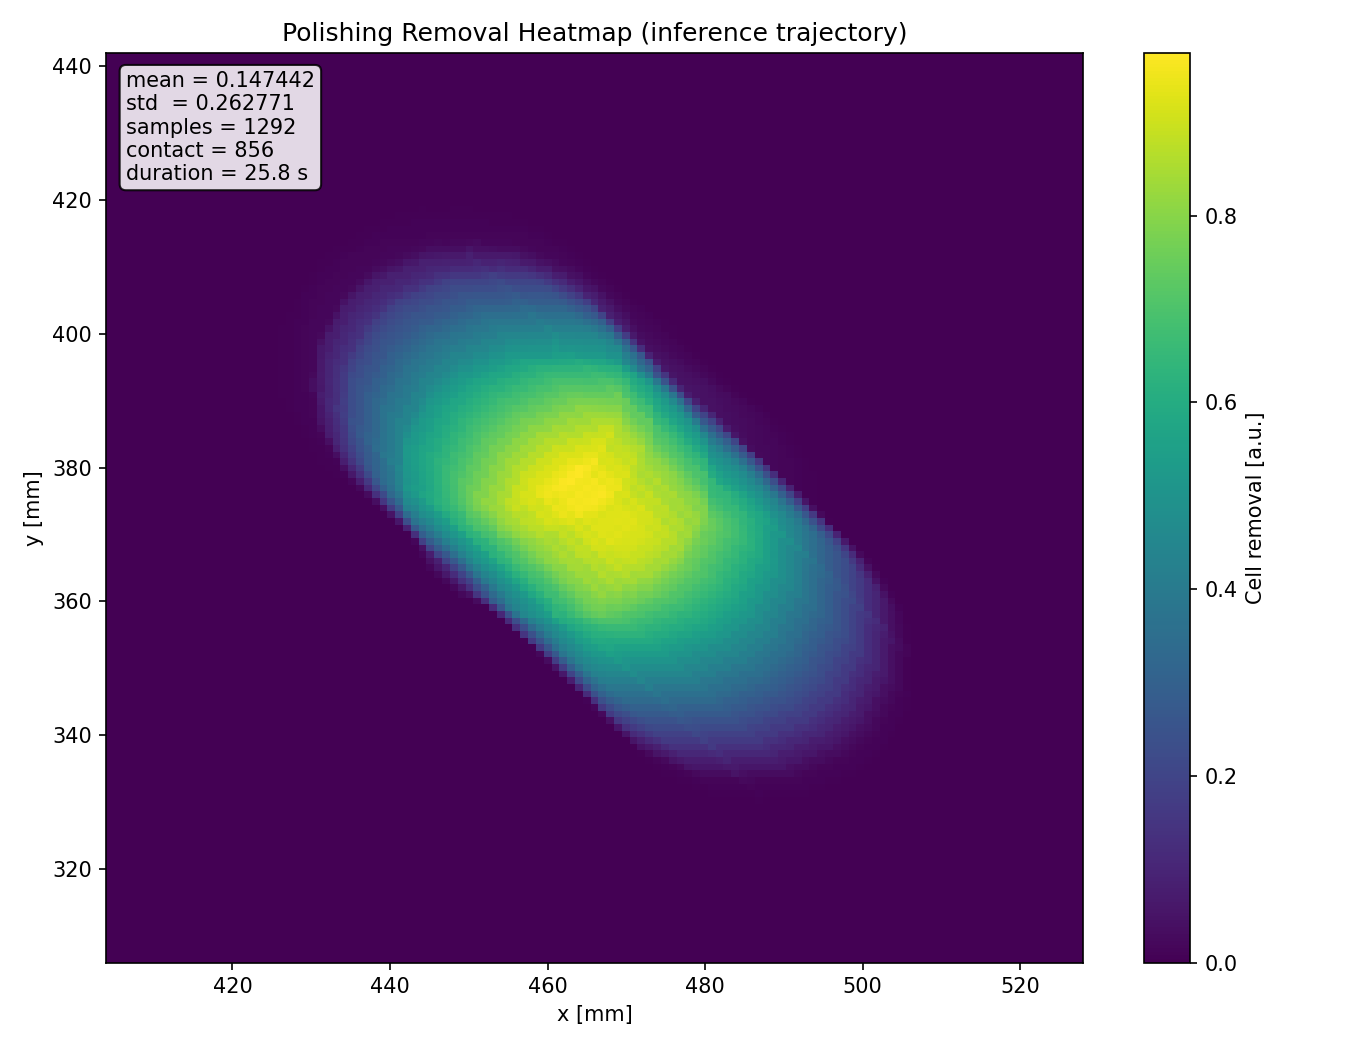
\includegraphics[width=\linewidth]{figures/E1_C1_diagnostic_heatmap.png}
\caption[Uncalibrated execution heatmap]{Existing execution-derived heatmap from E1 C1, reproduced with its original axes and colorbar. Values are an uncalibrated model diagnostic in arbitrary units. They are not measured removal depth, effective contact footprint, or surface-quality improvement. This figure is outside the primary E1 success measure.}
\label{fig:diagnostic_heatmap}
\end{figure}

The implementation and generated artifact support calling this an implemented diagnostic extension. They do not support the older claim of a calibrated material-removal model. Its spatial distribution may help inspect where modeled processing exposure accumulated, but equal dose is not demonstrated equal removal on the actual specimen.

\section{Blending and Adaptive Execution Assets}
\label{chap:blending}
The project also contains finite local blending-path generation from an existing dose map, construction of an additional spatial target, and time allocation along a path. The 13 October extension prepares a sequence in which an initial skill is followed by a separate blending pass and diagnostic displays. Its archived validation includes offline planning from an earlier execution. That is evidence of an implemented extension, not an E1/E2 surface-uniformity result.

Separate 14 October adaptive-velocity records provide development experience with reference-clock progression and replanning. The located runtime files contain five online-OFF development attempts across multiple versions. Their completion status does not establish a controlled adaptive ON/OFF process-quality comparison. A later source revision addresses a recorded stalled reference-clock case, but its README explicitly distinguishes offline checking from a new physical run. These records are therefore kept outside the nominal E2 A/B/C cohort.

\begin{table}[tbp]\centering\small
\caption[Status of inherited extensions]{Status of inherited extensions relative to the main thesis evidence.}
\label{tab:extension_status}
\begin{tabularx}{\textwidth}{P{0.32\textwidth}X}
\toprule Asset & Supported status \\ \midrule
Execution heatmap & Implemented and generated from runs; uncalibrated arbitrary-unit diagnostic. \\
Finite blending planner & Implemented; archived offline planning and integration preparation. Surface-quality improvement not established by the main comparisons. \\
Adaptive reference-clock execution & Separate versioned development attempts and code; controlled ON/OFF outcome benefit not established. \\
High-level residual RL for curved-surface restoration & Planned extension; completed skill-level training and quality-grounded evaluation not established in the selected evidence. \\
\bottomrule
\end{tabularx}
\end{table}

An earlier thesis concept proposed residual adjustments to orientation and feed velocity based on residual removal demand. That concept remains a possible extension, with its old formulation retained in the preserved source. Existing low-level learned mass/damping control is a different asset and does not validate that proposed high-level policy. The core motion--force skill in this thesis does not require a removal estimator, blending planner, or residual RL stage to count as an executable system.

\section{Limitations and Next Empirical Steps}
The immediate empirical limit is breadth. The nominal task and one trained seed per condition support a bounded comparison. Quantifying the implemented direction-transfer mechanism requires separately identified registration angles, active transfer settings, and task outcomes; E1/E2 supply no such comparison. Physical height changes, new shapes, operators, and tooling changes also require separately identified data. The prepared height protocol is the closest continuation of RQ1 because it tests an already stated research question without treating software preparation as a result.

Evaluation recognition also matters. The height-only replay demonstrates sensitivity to the initial reference, while the revised observer requires new receipt-event evidence. Future records should retain the evaluator version and observation support so that a physical strategy and its recognition can be assessed separately. Outcome corrections should remain additional interpretation records, as for A4, rather than edits to the original events.

Process-quality validation requires independent surface measurements with material and tooling records. Force-tracking validation instead requires synchronized controller-applied targets in a common frame. Neither measurement can be replaced by procedural completion.

\chapter{Conclusions}
\label{chap:conclusions}

Local robotic polishing requires a strategy for movement, contact loading, and time within a selected region. Human region specification supplies the spatial task, but does not by itself determine that temporal strategy. This thesis has addressed the resulting skill-generation problem through paired motion--force teaching, observation-conditioned sequence learning, and a common robot execution interface.

Tool position is learned relative to a frozen stain center and paired with orientation and target force on a shared sequence. The direction-transfer adapter aligns live XY and the policy image with the teaching direction, then restores generated XY by inverse rotation and center addition. Z, tool orientation, and force keep their conventions. The evaluated Flow Matching policy uses RGB, Cartesian state, and three-axis force history, with explicit coordinate restoration, pose conditioning, plan connection, and existing contact regulation. E1/E2 disable direction alignment and do not measure its transfer performance. The implementation separates upper-level skill generation, lower-level contact control, and completion recognition.

The first research question compares strategy providers. In the recorded E1 nominal cohort, rules, teaching replay, and the conditioned policy all show the required loaded ordered pass. The original completion counts differ, but the height-reference sensitivity analysis shows that the difference cannot be interpreted directly as a physical exit advantage for the policy. Replay provides a fast, repeatable nominal strategy, and the conditioned policy has greater excess-force exposure in this comparison. The implemented system therefore supports learning as an executable option alongside strong fixed alternatives; the current results do not establish its overall superiority. Performance under actual specimen-height changes remains unevaluated.

The second research question separates force output learning from force observation. E2 exercises all three implemented contracts while retaining lower-level feedback. The force-observing condition has shorter recorded operator-based completion intervals in this cohort, while A4 in the motion-only condition fails to progress to release and is interrupted. That attempt remains in the condition's five-attempt force and timing statistics, with successful completion time defined only for the other four attempts. These results reveal differences in phase progression and execution dispersion. The ordered, small, single-seed comparison does not isolate a universal causal advantage of either force-information choice.

The demonstrated scope is the generation and execution of a human-guided local contact skill on the marked-surface setup. It does not include autonomous recognition of defect severity, learned recognition of complete scratch removal, calibrated material-removal estimation, or measured surface restoration. The existing dose, blending, and adaptive-execution assets provide concrete extension paths, with their implementation and validation status stated separately from the main findings.

The thesis's contribution is the coherent connection from local task specification to a time-related motion--force representation, conditioned generation, shared execution, and corresponding evaluation. That connection provides a basis for deciding when rules or replay suffice and for testing, with additional physical conditions and quality measurements, when learned generation adds useful capability.

\clearpage
\bibliographystyle{IEEEtran}\bibliography{Bibliography/ThesisRef}
\setlinespacing{1.44}
\appendix
\chapter{Coordinates, Signals, and Reproduction}
\label{chap:appendix}
\label{app:signals}

\section{Pose and Force Signal Definitions}
The position vector is expressed in millimeters and orientation as a rotation vector in radians. The matrix \(R=\operatorname{Exp}([\rho]_\times)\) maps a vector in the calibrated tool frame to the robot base when it represents \(R_{B\leftarrow E}\). \([\rho]_\times\) is the skew-symmetric matrix associated with \(\rho\). The saved dataset transformation subtracts only \((c_x,c_y)\). The optional inference transformation additionally rotates center-relative XY by \(R_2(\alpha)\), with inverse rotation followed by center addition on output (Section~\ref{sec:stain_relative_generalization}). Both retain Z, tool rotation vectors, and force channels. The evaluated E1/E2 settings use \(\alpha=0\).

Teaching force is a three-component post-publisher measurement. Its associated tool orientation supplies the base-axis rotation in Equation~\eqref{eq:normal_force_projection}. Robot wrench feedback is already base expressed. A torque reference-point transformation would require a moment arm, but no torque transfer is needed for the three-force-component base projection used here. The available analysis does not infer a calibrated compliant contact point from a TCP-center trajectory.

\begin{table}[tbp]\centering\small
\caption[Force signal definitions]{Force signal roles used throughout the thesis.}
\label{tab:force_roles}
\begin{tabularx}{\textwidth}{P{0.31\textwidth}X}
\toprule Signal & Interpretation \\ \midrule
Teaching intention & Operator's approximate loading intention; not a numeric command trace. \\
Teaching recorded force & Measured interaction after the published processing path; used to construct learning supervision. \\
Policy force action & Denormalized output of the generator before executor gating and slew. \\
Executor transmitted target & Command-side force after shared processing; tangential target channels disabled in these comparisons. \\
Controller-applied reference & Target after internal controller processing; synchronized trace unavailable. \\
Robot measured force & Processed base-frame feedback used by the common gate, policy adapter, and recorded analysis. \\
\bottomrule
\end{tabularx}
\end{table}

\section{Learning and Temporal Parameters}
The force-cleanup dataset contains 15,963 paired frames in 42 compact episodes. The optimization and validation sets contain 38 and four episodes. Validation episode identifiers are 35, 39, 22, and 37. Each epoch's training window construction uses 50 starts per episode, a 128-step target, and the archived phase-sampling weights. The partition stored in each normalizer matches the dataset manifest.

The force-history dimension is three, its sample count is 30, and the selected recurrent layer is a one-layer GRU with hidden size 64. The state encoder receives pose and current force together in B/C. A removes the force state dimensions and history encoder. B retains the history architecture with zeroed conditioning. Physical force remains available to common execution in all conditions.

The training horizon, reference stride, inference timer, command period, and logging cap describe different mechanisms:
\begin{table}[tbp]\centering\small
\caption[Distinct clocks and sampling settings]{Distinct clocks and sampling settings.}
\label{tab:clock_definitions}
\begin{tabularx}{\textwidth}{P{0.39\textwidth}X}
\toprule Mechanism & Value or meaning \\ \midrule
Teaching paired sample grid & Nominal 30 Hz; original receipt times retained in merged HDF5. \\
Action sequence & 128 samples, nominal 30 Hz. \\
Nominal new-plan stride & 120 action samples, approximately 4 s. \\
Inference callback timer & 5 Hz, subject to plan-age gating. \\
Flow integration & 10 dimensionless updates per generated chunk. \\
Command publication & Nominal 125 Hz (0.008 s). \\
Feedback CSV logging & 20 Hz cap; approximately 18 Hz observed. \\
Analysis support & Receipt-time ZOH force and within-support pose interpolation; maximum gap 0.2 s. \\
\bottomrule
\end{tabularx}
\end{table}

\section{Reproducing the Manuscript and Figures}
The revised project is independent of the original thesis outputs. Its build retains the original pdfLaTeX/KoTeX/BibTeX chain and copies the existing school style without editing it. The body retains equal top and bottom margins of 25 mm. The cover remains a draft because the source did not establish author, adviser, committee, or submission details.

From this revised project directory, the full manuscript and separate cover are built with
\begin{verbatim}
bash build.sh
\end{verbatim}
The figures and tables can be regenerated from the bundled extracted data without the robot repository:
\begin{verbatim}
python3 scripts/plot_figures.py
python3 scripts/make_tables.py
bash build.sh
\end{verbatim}
The optional evidence-collection script rereads the original experiment files and writes only into this thesis directory. It contains no ROS initialization, robot commands, or training procedure. Its input manifest records SHA-256 values. The bundled data are extracts for publication and numerical reproduction; the source logs remain authoritative.

The figure manifest records original files, run identifiers, frame indices or video offsets, transformations, and manuscript locations. Conceptual diagrams reside in the chapter LaTeX and are distinguished from measured plots in their captions. No generated photograph is used.

\chapter{Experiment Versions and Provenance}
\label{app:provenance}

\section{Selected Models and Dataset}
The dataset and models are the force-cleanup revision dated 12 October, with training completed on 13 October 2026. All three selected checkpoints have their own normalizer. The best epochs are 39, 42, and 42, while final epoch is 499. The stored checkpoint selection rule is minimum validation loss over 500 epochs. Checkpoint metadata was read on CPU without policy execution or retraining.

\begin{table}[tbp]\centering\small
\caption[Selected model identifiers]{Short SHA-256 identifiers of the selected checkpoints and normalizers. Complete values are included in the supplied model manifest.}
\label{tab:model_provenance}
\begin{tabular}{lll}
\toprule Model & Checkpoint prefix & Normalizer prefix \\ \midrule
A & \texttt{2ea204ab65fb} & \texttt{ae7d07adf65a} \\
B & \texttt{080103e6c2ed} & \texttt{d7c917b8246c} \\
C & \texttt{60d55e7092cb} & \texttt{09111fa4acc3} \\
\bottomrule
\end{tabular}
\end{table}

The compact replay episode is linked to the source merged HDF5 recorded at 16:18 on 19 August 2026, source episode \texttt{ep\_0003}. Its compact action and observation pose/force arrays contain 443 frames. The original source-time array is retained for T rather than replaced by an assumed constant period. The exact source paths and extraction fields are recorded in the supplied episode metadata.

\section{E1 Versions}
The executed nominal cohort is
\begin{quote}\small\path{E1_CT_sync_confirm_dev_20261014}\end{quote}
with configuration version \texttt{e1ct\_61a19f7d7337a82c}. Its frozen task evaluation uses the initial-contact height reference. Its development status and method order are retained. Although there is an approximately 172 mm surface-reference value in configuration, the actual per-trial physical setup field is not recorded precisely. This nominal label is not a measurement of specimen height.

The height-only replay is found under
\begin{quote}\small\path{reports/E1_contact_task_pass_height_v2/baseline_replay/}\end{quote}
and changes the release-height reference on the stored observation stream. Its report columns A/B/C refer to analysis variants, not the A/B/C learned conditions of E2 or method C. The thesis calls them original evaluation, height-only replay, and revised-observer reconstruction to avoid that ambiguity.

The revised nominal session and the two prepared physical-height session versions have empty attempt lists at the evidence cutoff. Their existence establishes preparation. It does not establish a robot execution or a successful revised-observer comparison. The status snapshot is supplied as \path{provenance/height_session_status.json}.

\section{E2 Versions and the A4 Correction}
The selected E2 cohort uses the force-cleanup revision of 13 October. Each actual \texttt{runtime.json} names its model revision, observation settings, and common executor. The run inventory orders the attempts A1--A5, B1--B5, and C1--C5. Preparation-only runtime files are not used as substitutes for these actual run files.

The old E2 report applied a common operator-confirmed completion interpretation to all 15 attempts. The later task instruction specifically corrects A4. This thesis adopts that field correction and stores it in \path{data/e2_operator_correction.json}. The original software event remains \texttt{operator\_finish}, followed by the original normal-completion stop-path event. The derived task outcome is separately marked incomplete contact release. The original elapsed time 28.750087346 s remains the interruption interval.

The correction changes only the successful-time aggregation and task interpretation. A4 remains in all five-attempt statistics for force, travel, and elapsed interval. No surface image, raw force sample, event timestamp, or checkpoint is edited. The corrected table can be reconstructed from \path{data/e2_runs_corrected.csv}.

\section{Sources for Implemented Extensions}
The execution heatmap is generated by the existing polishing-removal recorder. The finite blending path and dose tools are in the local blending module and the 13 October extension package. The adaptive-velocity development records are versioned separately under the 14 October results directory. Their runtime metadata identifies them as adaptive-execution development rather than the primary E2 force ablation.

The selected-source directory preserves small source/configuration copies used in the methods, including the training Flow policy, dataset construction, the historical timed executor/evaluator, force correspondence notes, calibration parameters, and the existing controller implementation. These files are reading evidence. They are not a replacement robot project, and no robot-side modification is part of this thesis revision.

\chapter{Individual Outcomes and Update Locations}
\label{app:runs}

\section{E1 Started Executions}
Table~\ref{tab:e1_all} lists the complete started cohort. All 15 have an observed loaded pass through 14 ordered segments. The three incomplete classifications refer to the original exit criterion. A missing time indicates no completion under that criterion.

\begin{table}[tbp]\centering\small
\caption[Individual E1 outcomes]{Individual E1 original-criterion outcomes. Every listed execution is retained. Full run identifiers and original directories are in the accompanying CSV inventory.}
\label{tab:e1_all}\begin{tabular}{llrr}
\toprule
Run & Procedural outcome & Time (s) & $J_{\mathrm{excess}}$ (N\,s) \\
\midrule
R1 & incomplete & \NA & 0.0000 \\
R2 & completed & 29.544 & 0.0000 \\
R3 & incomplete & \NA & 0.0000 \\
R4 & completed & 29.587 & 0.0000 \\
R5 & completed & 29.607 & 0.0000 \\
T1 & completed & 12.869 & 0.0237 \\
T2 & completed & 12.858 & 0.0000 \\
T3 & completed & 12.865 & 0.0000 \\
T4 & incomplete & \NA & 0.0000 \\
T5 & completed & 12.843 & 0.0000 \\
C1 & completed & 16.764 & 0.7121 \\
C2 & completed & 19.954 & 5.4212 \\
C3 & completed & 11.954 & 0.3246 \\
C4 & completed & 17.751 & 4.6456 \\
C5 & completed & 11.919 & 0.5106 \\
\bottomrule
\end{tabular}

\end{table}

The additional original R5 registration is
\begin{quote}\footnotesize\path{E1_CT_NOMINAL_R_r5_20261014T191508_af5aecaa94}.\end{quote}
It is classified as not started and has no physical trajectory-based completion or force result. Its subsequent retry is
\begin{quote}\footnotesize\path{E1_CT_NOMINAL_R_r5_20261014T191842_b6bc0bbdb3}.\end{quote}
That retry is the started R5 in Table~\ref{tab:e1_all}. The primary completion denominators are five started trials per method. For bookkeeping over all registrations, R has six registrations, five starts, and three original-criterion completions; this denominator is distinct from the started-execution rate. The source exclusion record is preserved as a provenance file without deleting the original registration.

\section{E2 All Attempts}
Table~\ref{tab:e2_all} distinguishes successful completion intervals from time to interruption. All original stop requests are retained. In particular, the missing A4 completion time is not a missing raw record.

\begin{table}[tbp]\centering\small
\caption[Individual E2 corrected task outcomes]{Individual E2 task outcomes after the A4 field correction. ``Operator completed'' uses the recorded operator interpretation; it is not an automatic E1 evaluation.}
\label{tab:e2_all}\begin{tabular}{llrr}
\toprule
Run & Task outcome & Completion (s) & Interval to stop (s) \\
\midrule
A1 & operator completed & 16.787 & 16.787 \\
A2 & operator completed & 16.445 & 16.445 \\
A3 & operator completed & 18.581 & 18.581 \\
A4 & interrupted & \NA & 28.750 \\
A5 & operator completed & 18.777 & 18.777 \\
B1 & operator completed & 18.690 & 18.690 \\
B2 & operator completed & 18.511 & 18.511 \\
B3 & operator completed & 19.508 & 19.508 \\
B4 & operator completed & 18.693 & 18.693 \\
B5 & operator completed & 18.671 & 18.671 \\
C1 & operator completed & 15.902 & 15.902 \\
C2 & operator completed & 15.297 & 15.297 \\
C3 & operator completed & 15.597 & 15.597 \\
C4 & operator completed & 16.751 & 16.751 \\
C5 & operator completed & 15.618 & 15.618 \\
\bottomrule
\end{tabular}

\end{table}

The archived video inventory contains B/C videos but no A videos. The illustrated C1 WebM has an incomplete container ending; only decodable frames are used. It is not treated as a continuous independent proof of full task completion. Snapshot timing and varying tool viewpoint also limit before/after interpretation.

\section{Updating the Thesis without Mixing Cohorts}
Future physical NOMINAL/LOW/HIGH results belong in a separate subsection of Chapter~\ref{chap:experiments}, with their actual session, evaluation/observer version, model identifiers, and physical placement records. The existing original-criterion table and height-only replay remain historical comparisons. Their numbers should not be overwritten to imply the revised evaluator ran on the robot.

New A/B/C data similarly require their own cohort table if the model, force preprocessing, executor, observation convention, or stopping interpretation changes. A measured surface-quality study belongs beside the contact-procedure evaluation with its own metrology and processing conditions. Confirmed blending or high-level residual-policy results would expand Chapter~\ref{chap:discussion}, while preserving the separation from the motion--force skill results established here.

\chapter*{국문요약}
\addcontentsline{toc}{chapter}{국문요약}
\begin{center}\large\bfseries\thesistitlekr\end{center}

표면 마무리 공정에서 부품 전체의 균일 처리와 지정된 영역 주변의 국소 재작업은 서로 다른 요구를 가진다. 국소 폴리싱에서는 대상 영역에 맞추어 공구 이동, 접촉 힘, 작업 시간을 함께 구성해야 한다. 본 연구는 현재 장비로 미세 스크래치를 자율 판별하는 대신 사람이 처리 영역을 지정하는 설정을 사용한다. 공간 지시 이후에도 남는 동작·힘·시간 구성 문제에 대해, 규칙 기반 전략과 교시 재생에 비해 관측 조건부 학습이 어떤 수행 가치를 추가하는지 검토한다.

추적 기반 교시 장치로 공구 위치·자세, 3축 힘, RGB 영상을 시간적으로 대응하여 기록한다. 얼룩 중심 상대위치를 학습하고 얼룩 방향을 학습 기준에 정렬한다. Flow Matching 정책은 영상, 로봇 상태, 측정 힘 이력으로 위치·자세·목표 힘 시퀀스를 생성한다. 공통 실행 계층은 좌표 복원, 계획 연결, 명령 후처리를 수행하고 기존 하위 힘제어기가 접촉을 조절한다. 스킬 생성, 접촉 제어, 절차 완료 판정의 역할을 분리한다.

E1/E2는 방향 정규화 없이 평가한다. E1은 기준조건에서 규칙 기반 경로, 힘을 포함한 교시 재생, 힘 조건부 정책을 비교한다. 모든 실행에서 요구된 부하 편도 통과가 관측되었다. 기존 완료율 차이는 상승 이탈의 높이 기준에 민감하였고, 학습 정책의 초과 힘 적분은 다른 방법보다 컸다. 동일 기록으로 판정 민감도를 분석하고 실제 시편 높이 변화 시험은 계획으로 구분하였다. E2는 목표 힘 학습과 측정 힘 관측을 분리한다. 힘 관측 정책의 작업자 종료 구간이 더 짧았으나, 동작만 학습한 조건의 한 시행은 접촉 해제로 전환하지 못해 작업자가 중단하였다. 결과는 동작--힘 표현의 실행 가능성과 단계 진행의 차이를 보여주며, 정책의 보편적 우위나 표면 품질 향상을 입증하지는 않는다. 본 연구는 국소 작업에서 규칙·재생·학습의 활용 범위를 검토할 수 있는 구현과 평가 근거를 제공한다.

\vspace{0.4cm}
\noindent\textbf{주요어:} 국소 로봇 폴리싱, 인간 작업 지정, 동작--힘 스킬, 모방학습, Flow Matching, 접촉 작업 평가

\end{document}
